\documentclass[11pt,reqno]{amsart}
\usepackage[T1]{fontenc}
\usepackage{lmodern,amsmath,amssymb,amsthm,mathtools,microtype}
\usepackage[a4paper,margin=28mm]{geometry}
\usepackage{tikz,booktabs,array,enumitem,xcolor}
\usetikzlibrary{arrows.meta,positioning,calc,patterns}
\usepackage[colorlinks=true,linkcolor=blue!45!black,citecolor=blue!45!black,urlcolor=blue!45!black]{hyperref}
\usepackage[nameinlink,noabbrev]{cleveref}
\numberwithin{equation}{section}
\newtheorem{theorem}{Theorem}[section]
\newtheorem{proposition}[theorem]{Proposition}
\newtheorem{lemma}[theorem]{Lemma}
\newtheorem{corollary}[theorem]{Corollary}
\theoremstyle{definition}
\newtheorem{definition}[theorem]{Definition}
\newtheorem{example}[theorem]{Example}
\theoremstyle{remark}
\newtheorem{remark}[theorem]{Remark}
\newcommand{\Tr}{\operatorname{Tr}}
\newcommand{\supp}{\operatorname{supp}}
\newcommand{\diam}{\operatorname{diam}}
\newcommand{\dist}{\operatorname{dist}}
\newcommand{\TV}{\operatorname{TV}}
\newcommand{\Id}{\operatorname{Id}}
\newcommand{\ad}{\operatorname{ad}}
\newcommand{\poly}{\operatorname{poly}}
\newcommand{\rank}{\operatorname{rank}}
\newcommand{\E}{\mathbb E}
\newcommand{\Prb}{\mathbb P}
\newcommand{\C}{\mathbb C}
\newcommand{\Z}{\mathbb Z}
\newcommand{\R}{\mathbb R}
\newcommand{\nn}[1]{\lVert#1\rVert}
\newcommand{\abs}[1]{\lvert#1\rvert}
\newcommand{\ip}[2]{\langle#1,#2\rangle}
\newcommand{\ket}[1]{\lvert#1\rangle}
\newcommand{\bra}[1]{\langle#1\rvert}
\newcommand{\reset}{\mathcal R}
\newcommand{\cL}{\mathcal L}
\newcommand{\cG}{\mathcal G}
\newcommand{\cN}{\mathcal N}
\setlist[enumerate]{label=\textup{(\roman*)},leftmargin=*,itemsep=3pt}
\setlist[itemize]{leftmargin=*,itemsep=3pt}
\hypersetup{pdftitle={Global Readouts of Noisy Quantum Dynamics},pdfauthor={Harjas Sandhu}}
\title[Global readouts of noisy quantum dynamics]{Global Readouts of Noisy Quantum Dynamics}
\author{Harjas Sandhu}
\address{The University of Queensland}
\email{harjas.sandhu@student.uq.edu.au}
\date{8 November 2026}
\subjclass[2020]{Primary 81P68; Secondary 81P45, 82C10, 68Q17}
\keywords{open quantum systems, classical simulation, hypercontractivity, product observables, replacement noise, tensor networks, system identification}
\begin{document}
\raggedbottom
\begin{abstract}
We give a randomized polynomial-time classical algorithm for additive prediction of arbitrary products of one-qubit Hermitian contractions in a driven two-dimensional quantum system. Every qubit undergoes replacement at a fixed positive rate. The replacement state may be biased and full rank, provided that the Hamiltonian preserves its product reference; maximally mixed replacement imposes no conservation restriction. The input is a specified product state, the controls have an explicit finite rational description, and the complexity is polynomial in the complete binary input, inverse error and confidence digits, at each fixed positive noise ratio and faithfulness bound. The proof combines coefficient sparsification with a constructible short-time functional: two localized strip states, including retained reset registers, have polynomial Schmidt nuclear norm and admit bounded overlap estimation. Moving coefficient weights and weighted hypercontractivity extend local prediction to readouts of unrestricted support. We also prove a full-output sampler under a supplied bounded-cut certificate, give an acquired-model prediction theorem with explicit uncertainty and preparation costs, and identify two boundaries: rare-probability evaluation remains conditionally hard, and exponentially accurate product means need not determine a distribution in total variation. General intermediate-time two-dimensional output sampling remains open.
\end{abstract}
\maketitle
\setcounter{tocdepth}{1}
\tableofcontents
\clearpage
% BEGIN sections/overview
\section{Conceptual overview: a computable boundary functional}\label{sec:overview}

Think of the observable as moving backward from the final measurement towards the preparation. Noise suppresses complicated coefficient patterns. The remaining difficulty is evaluating those patterns on a specific source, rather than on an average over sources.

\begin{center}
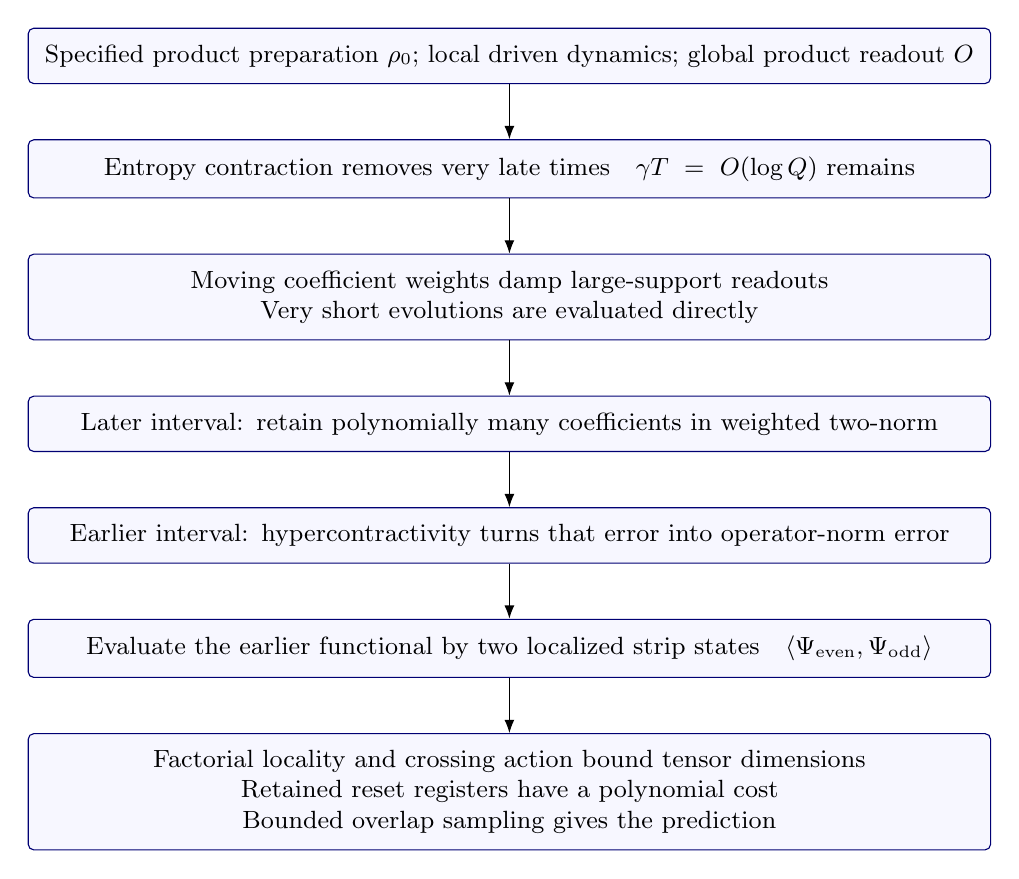
\begin{tikzpicture}[>=Latex,node distance=7mm,box/.style={draw=blue!45!black,rounded corners=2pt,fill=blue!3,text width=11.8cm,align=center,inner sep=6pt,font=\small}]
\node[box] (a) {Specified product preparation $\rho_0$; local driven dynamics; global product readout $O$};
\node[box,below=of a] (b) {Entropy contraction removes very late times\quad $\gamma T=O(\log Q)$ remains};
\node[box,below=of b] (c) {Moving coefficient weights damp large-support readouts\\Very short evolutions are evaluated directly};
\node[box,below=of c] (d) {Later interval: retain polynomially many coefficients in weighted two-norm};
\node[box,below=of d] (e) {Earlier interval: hypercontractivity turns that error into operator-norm error};
\node[box,below=of e] (f) {Evaluate the earlier functional by two localized strip states\quad $\langle\Psi_{\rm even},\Psi_{\rm odd}\rangle$};
\node[box,below=of f] (g) {Factorial locality and crossing action bound tensor dimensions\\Retained reset registers have a polynomial cost\\Bounded overlap sampling gives the prediction};
\foreach \u/\v in {a/b,b/c,c/d,d/e,e/f,f/g} \draw[->] (\u)--(\v);
\end{tikzpicture}
\end{center}

The early and later intervals have different roles. A small coefficient error is created on the later interval. The actual earlier channel smooths that error. The earlier channel must also be evaluated; the strip construction performs this operation without moving it through the drive.

The crucial balance is geometric. For a short duration $t=O(\log\log Q)$, a factorial light cone needs strip width $b=O(\log Q/\log\log Q)$. Across a horizontal cut, the sum of Schmidt coefficients grows at most as $\exp(CbJt)=Q^{O(1)}$. That bound supports an explicit compression algorithm. Biased replacement is represented by swapping in a sampled local reset state and keeping the old register. A concentration bound limits the added row dimension at a paid expectation-error cost. Finally, a bounded importance sampler estimates the overlap even though the two strip states have different natural tensor orderings.

The outcome is a scalar prediction with a confidence interval. A sampler for all measurement outcomes requires additional positive, jointly consistent information. The bounded-cut theorem supplies it in a restricted architecture; the general two-dimensional problem remains separate.

% END sections/overview

\clearpage
% BEGIN sections/introduction
\section{Introduction}

Noise erases information, but it does not immediately make quantum dynamics easy to predict. Before equilibration, a local Hamiltonian can distribute information over many sites. Even a compact approximation to a Heisenberg observable may be inadequate for a specified initial state: a small Hilbert--Schmidt error can have a large expectation on that state. A useful simulation theorem must therefore control both the propagated observable and the functional that evaluates it.

This paper studies that issue for a concrete dissipative model. Qubits occupy a finite region of the square lattice, interact through bounded-range Hamiltonian blocks, and are independently replaced by the same known qubit state at rate $\gamma>0$. Coherent controls are permitted throughout the evolution. For unbiased replacement the controls are arbitrary within the local bounds. For biased replacement they must conserve the product reference state. The question is pointwise: given a particular product preparation, a particular drive and a particular product readout, can its final mean be computed efficiently at every fixed positive noise-to-interaction ratio?

\Cref{thm:main} answers this question affirmatively for additive accuracy. The readout may occupy the entire system. It includes parity, correlations between distant spins, and the probability of a specified product-projector event. The running time is polynomial in inverse additive error, rather than in its logarithm. Consequently, exponentially rare events do not acquire relative accuracy from this statement. The polynomial degree depends on the fixed noise ratio and on a lower bound for the eigenvalues of the replacement state.

\subsection{The missing operation}
Sparse coefficient propagation supplies an important part of the answer. Angrisani, Puig, Teng and Holmes prove coefficient contraction and sparse Hilbert--Schmidt propagation for dissipative dynamics \cite{APTH}. Their operational average-case guarantees retain their stated quantifiers. A Hilbert--Schmidt approximation alone does not give the specified-input theorem considered here. For example, on $m$ qubits the rank-one projector $\ket{0^m}\bra{0^m}$ has normalized Hilbert--Schmidt norm $2^{-m/2}$ but expectation one in $\ket{0^m}$.

Hypercontractivity can convert the coefficient error into operator-norm error after a short additional evolution. This leaves a computational task: evaluate the resulting short-time functional on a specified product source. We construct that functional. Its duration grows as $O(\log\log Q)$, where $Q$ measures the complete instance and inverse accuracy. The construction pays its numerical precision, tensor dimensions, random bits and, for biased resets, the discarded local registers that must be retained in a unitary representation. It does not introduce an extra physical preparation or cooling operation.

The global-readout extension requires a further step. A product with many traceless factors is strongly attenuated, but those factors need not be centered in a biased reference. A moving weight in coefficient space, followed by Hamiltonian-sign duality, gives a support-sensitive estimate that survives this distinction. That estimate separates the problem into a directly constructible early-time branch, a negligible high-support branch, and a sparse low-support branch.

\subsection{Relation to existing methods}
The short-time representation builds on the two-strip-state overlap architecture of Bravyi, Gosset and Movassagh \cite[Theorem~5]{BGM}. Their theorem concerns a shallow circuit. Substituting the number of time-discretization layers for its depth would not give a continuous-time polynomial bound. Here the relevant quantity is the accumulated interaction strength across a cut. A factorial locality estimate, in the form developed by Haah, Hastings, Kothari and Low \cite[Lemma~5 and Appendix~C.4]{HHKL}, then makes the product of strip width and physical duration logarithmic in $Q$.

The analytic smoothing is established machinery: King gives tensorized unital-qubit hypercontractivity \cite[Theorem~1 and Corollary~2]{King}; Beigi, Datta and Rouz\'e develop weighted qubit inequalities \cite[Theorems~21 and~25]{BDR}; and Dong, Gao, Ou, Yao and Zhou give the all-operator tensorized estimate used below \cite[Theorem~1.1]{DGOYZ}. We prove applicability to the actual time-dependent Hamiltonian by interleaving norm isometries, with no commutation of different time intervals.

There are stronger sampling results under different hypotheses. Trivedi and Cirac state a high-noise continuous-time sampling theorem \cite[Theorem~1]{TC}. Nelson, Rajakumar, Yin, Zhang and Gullans give a polynomial sampler, and stronger marginal guarantees, for discrete unital circuits above a noise-dependent depth \cite[Theorem~2.3 and Proposition~2.2]{NR}. The latter assumes a fixed depolarizing strength per layer. Under a fine time discretization that strength is $O(\gamma h)$; its threshold and degree are not uniform as $h\downarrow0$. Constructive whole-trajectory positive matrix-product approximations are also known for one-dimensional circuits with fixed per-layer noise \cite[Propositions~1 and~4]{Shao}. These results are not used as black-box proofs of our all-ratio two-dimensional continuous-time theorem. Parameter-averaged nonunital simulation \cite{Martinez} and random-layer guarantees \cite{AMRCH} likewise do not give a pointwise theorem for every prescribed conserving drive.

\subsection{Contributions and organization}
The main contribution is the specified-input global-readout algorithm, including the faithful biased-reset construction. Sections~\ref{sec:analytic}--\ref{sec:assembly} give its proof. The two reusable operations are stated separately: a positive short-buffer evaluator and a moving-weight sparse reduction. Sections~\ref{sec:sampling} and~\ref{sec:acquisition} develop consequences with additional geometric or experimental access assumptions. Section~\ref{sec:obstructions} proves limits on relative probabilities and on converting scalar predictions into a sampler. These consequences use established tensor-network, stability and learning methods where appropriate; their value here is a complete composition with an efficient evaluator.

% END sections/introduction

% BEGIN sections/results
\section{Model and main theorem}\label{sec:results}

Let $\Lambda\subset\Z^2$ be an explicitly listed finite set of $n\geq1$ sites, with distance measured in the maximum metric. Holes and disconnected regions are allowed. Each site carries $\C^2$. Fix positive class parameters $a,k,d,g$ and $0<\nu\leq1/2$. During each segment of a supplied finite rational schedule,
\begin{equation}\label{eq:H}
 H(t)=\sum_b H_b(t),\qquad
 \abs{\supp H_b}\leq k,\quad \diam(\supp H_b)\leq a,\quad
 \nn{H_b}\leq J,
\end{equation}
and at most $d$ blocks meet a site. Blocks are Hermitian matrices with rational real and imaginary parts. The bounds $J,\gamma>0$ are rational and $J/\gamma\leq g$. All schedule segments, matrices, sites and switching times are explicitly charged.

Put $\sigma=\operatorname{diag}(p,1-p)$, where $p$ is rational and
$\mu:=\min(p,1-p)\geq\nu$. The Schr\"odinger evolution is
\begin{equation}\label{eq:model}
 \dot\rho_t=\cL_t(\rho_t),\qquad
 \cL_t(\rho)=-i[H(t),\rho]+\gamma\sum_{i\in\Lambda}(\reset_i(\rho)-\rho),
 \quad \reset_i(\rho)=\sigma_i\otimes\Tr_i\rho.
\end{equation}
Tensor factors are placed at their indicated sites. Assume
\begin{equation}\label{eq:conserve}
 [H(t),\Sigma]=0,\qquad \Sigma=\sigma^{\otimes n}.
\end{equation}
This assumption is automatic at $p=1/2$. When $p\ne1/2$ it is equivalent to conservation of the total number of excitations. The stationary reference $\Sigma$ is generally not the Gibbs state of the interacting Hamiltonian $H(t)$.

Write $\Phi_{s,t}$ for the Heisenberg propagator, so that
$\Tr(\rho_s\Phi_{s,t}A)=\Tr(\rho_tA)$ and
$\Phi_{s,t}=\Phi_{s,u}\Phi_{u,t}$. Its local reset is
$E_iA=I_i\otimes\Tr_i(\sigma_i A)$.

\begin{theorem}[Global product-readout prediction]\label{thm:main}
For the fixed class parameters above, there is a bounded-work randomized classical algorithm with the following contract. Supply the data in \eqref{eq:H}--\eqref{eq:conserve}, a rational product state $\rho_0=\bigotimes_i\rho_i$, a rational time $T\geq0$, and a product
\[
 O=\bigotimes_{i\in\Lambda}O_i,\qquad O_i=O_i^\dagger,\quad\nn{O_i}\leq1,
\]
with rational entries. For rational $0<\epsilon\leq1/2$ and $0<\delta<1$, the algorithm returns a rational number $\widehat f$ such that
\begin{equation}\label{eq:guarantee}
 \Prb\!\left\{\abs{\widehat f-\Tr(\rho_T O)}\leq\epsilon\right\}\geq1-\delta.
\end{equation}
Its bit work is polynomial in $B+n+\epsilon^{-1}+\log(2/\delta)$, where $B$ is the complete binary input length. The degree and prefactor depend only on $a,k,d,g,\nu$.
\end{theorem}

In particular, $T$ is paid in binary. The algorithm first tests whether equilibration makes dynamical evaluation unnecessary. The statement is not uniform as $\gamma/J\downarrow0$ or $\mu\downarrow0$. The supplied structural and positivity conditions are promises of the numerical problem; they can be checked in the fixed local matrix dimensions, apart from global promises already reduced below.

\begin{example}[Exchange interactions and a parity measurement]
Take
\[
 H(t)=\sum_{\langle i,j\rangle}
 \{u_{ij}(t)(X_iX_j+Y_iY_j)+v_{ij}(t)Z_iZ_j\}
 +\sum_i h_i(t)Z_i.
\]
With the bounds in \eqref{eq:H}, every block preserves $\sigma\otimes\sigma$ for any bias $p$. The theorem predicts $\langle\prod_{i\in S}Z_i\rangle$ for any specified $S$, including $S=\Lambda$, from any specified product preparation. It also predicts $\Pr\{x_i=1\text{ for all }i\in S\}$ additively, by taking $O_i=(I-Z_i)/2$. It does not resolve that probability to relative error when it is exponentially small.
\end{example}

\begin{lemma}[Conservation can be made local]\label{lem:twirl}
Under \eqref{eq:conserve}, the blocks may be replaced, constructively and without increasing their supports, norms or incidence, by blocks satisfying
$[H_b,\sigma^{\otimes\supp H_b}]=0$.
\end{lemma}
\begin{proof}
Only $p\ne1/2$ needs attention. Write $N=\sum_i(I-Z_i)/2$, so $\Sigma$ is a nonconstant exponential of $N$. Average each block over $e^{i\varphi N}$, $0\leq\varphi<2\pi$. On its support this deletes matrix entries between unequal excitation sectors. It is a rational, norm-contracting pinching in fixed dimension. The sum of the averages equals $H$ because $[H,N]=0$. The unbiased case needs no change.
\end{proof}

The proof below therefore uses reference-preserving whole blocks. Splitting such a block into individual Pauli Hamiltonians is not permitted in the sparse propagation step: its summands can fail to preserve $\sigma$. A Pauli expansion is used only in estimates where the approximation error is independently paid.

\subsection{What is supplied, and what is concluded}
The specified product source is essential. Arbitrary circuit-described inputs already contain hard computations at time zero. No additional physical reset or control operation is introduced by the algorithm. The random reset histories and purifications are classical representations of \eqref{eq:model}. Output clipping gives the usual interval $[\widehat f-\epsilon,\widehat f+\epsilon]\cap[-1,1]$ at the confidence in \eqref{eq:guarantee}. An arbitrary observable on a fixed number $w$ of sites is also covered: expand it into its at most $4^w$ Pauli products and divide the precision and confidence budgets over that fixed sum.

\Cref{thm:cuts} will add a supplied bounded-cut tree and earn a full-output total-variation sampler. \Cref{thm:service} will instead add experimental access to an unknown local drift and earn reusable predictions with explicit uncertainty. These are distinct extensions of the main theorem.

% END sections/results

% BEGIN sections/analytic
\section{Mixing, smoothing and physical support}\label{sec:analytic}

This section establishes estimates for the actual propagator. They do not depend on a numerical time step. All restrictions of the system retain the resets on the sites that remain, and retain only Hamiltonian blocks wholly contained in the restricted region.

\subsection{Entropy contraction and localization}
\begin{lemma}[Entropy cutoff]\label{lem:entropy}
For every initial state, including a correlated state,
\begin{equation}\label{eq:entropy}
 D(\rho_t\Vert\Sigma)\leq n\log(\mu^{-1})e^{-\gamma t},\qquad
 \nn{\rho_t-\Sigma}_1\leq\sqrt{2n\log(\mu^{-1})}\,e^{-\gamma t/2}.
\end{equation}
These inequalities hold for bounded time-dependent reference-preserving Hamiltonians.
\end{lemma}
\begin{proof}
The Hamiltonian contribution to the derivative of relative entropy is zero: the von Neumann entropy is invariant under conjugation and $[H,\log\Sigma]=0$. Convexity gives
\[
 dD(\rho\Vert\Sigma)[\reset_i\rho-\rho]
 \leq D(\reset_i\rho\Vert\Sigma)-D(\rho\Vert\Sigma).
\]
Writing the reference as a product shows
\[
 \sum_i\{D(\rho\Vert\Sigma)-D(\reset_i\rho\Vert\Sigma)\}
 =-nS(\rho)+\sum_iS(\rho_{-i})-\Tr(\rho\log\Sigma)
 \geq D(\rho\Vert\Sigma).
\]
The inequality is quantum Shearer's inequality, $\sum_iS(\rho_{-i})\geq(n-1)S(\rho)$. To see it, expand each entropy in the same site order by the chain rule. Removing a conditioning site increases conditional entropy by strong subadditivity; each full chain-rule term is counted $n-1$ times. Thus $\dot D\leq-\gamma D$. Initially $D\leq n\log(\mu^{-1})$. Integration and quantum Pinsker give \eqref{eq:entropy}. Regularizing the initial state and passing to the limit covers singular states.
\end{proof}

We use the following two locality forms. Constants denoted by $C$ below can be increased and depend only on the declared local parameters. They are computable from the interaction bounds.

\begin{lemma}[Two locality estimates]\label{lem:locality}
Let $A$ have norm at most one and support $S$, $r=|S|$. Restriction to the radius-$R$ neighborhood of $S$ gives
\begin{equation}\label{eq:LR}
 \nn{\Phi_{s,t}A-\Phi^{R}_{s,t}A}
 \leq Cr^2\exp\{C(J+\gamma)(t-s)-R/(2a)\}.
\end{equation}
In particular an error $\eta$ can be achieved using
\begin{equation}\label{eq:m}
 m\leq\min\{n,Cr[1+(J+\gamma)(t-s)+\log((r+1)/\eta)]^2\}
\end{equation}
actual lattice sites. For a unitary trajectory with arbitrary on-site permutations of internal registers and Hamiltonian action $Jt$, restriction across a buffer of $q$ interaction ranges instead obeys
\begin{equation}\label{eq:factorial}
 \nn{U^\dagger A U-U_B^\dagger A U_B}
 \leq C |S|e^{CJt}\frac{(CJt)^q}{q!}.
\end{equation}
The constants are independent of the number of internal registers and time steps.
\end{lemma}
\begin{proof}
For \eqref{eq:LR}, apply the local Lindblad truncation estimate of Barthel--Kliesch \cite[Theorems~1--2]{BK}. The local maps have norm at most $2J$ or $2\gamma$, bounded support and bounded incidence. A square-lattice shell has at most $Cr(\ell+1)$ sites, which satisfies their polynomial-growth hypothesis. Their time-dependent norm bound uses precisely the supremum local strengths here. Summing the boundary shells, enlarging constants and allowing the harmless quadratic support prefactor gives \eqref{eq:LR}. Choosing $R=O(a[1+(J+\gamma)(t-s)+\log((r+1)/\eta)])$ absorbs that prefactor. Counting sites in the union of $r$ balls gives \eqref{eq:m}; missing lattice sites are not filled.

For \eqref{eq:factorial}, move every on-site permutation into the toggling frame. This changes the internal register on which a block acts but leaves its spatial support and norm unchanged. The linked-interaction expansion of a commutator across the buffer requires at least $q$ successive overlapping blocks. The maximum sum of $|\supp H_b|\nn{H_b}$ at a site is at most $kdJ$. Ordered time integrals contribute $t^\ell/\ell!$. The linked-path estimate in \cite[Lemma~5, Appendix~C.4, (48)--(49)]{HHKL}, with this bound and the range-rescaled metric, gives the factorial tail; allowing the displayed $e^{CJt}$ absorbs the tail sum and boundary integration. The same ordered integrals apply to piecewise time-dependent blocks. Only spatial supports enter this argument, so internal dimension and on-site permutations do not alter it.
\end{proof}

\subsection{Weighted hypercontractivity and chronology}
For an $m$-site reference $\Sigma_m=\sigma^{\otimes m}$ define the symmetric weighted Schatten norm
\begin{equation}\label{eq:KMS}
 \nn{A}_{q,\Sigma_m}
 =\nn{\Sigma_m^{1/(2q)}A\Sigma_m^{1/(2q)}}_q,
 \qquad1\leq q<\infty,
\end{equation}
using the ordinary, unnormalized Schatten norm on the right. Thus $\nn{I}_{q,\Sigma_m}=1$. At $q=2$ its inner product is
$\ip AB_{\Sigma_m}=\Tr(A^\dagger\Sigma_m^{1/2}B\Sigma_m^{1/2})$. At $\sigma=I/2$, \eqref{eq:KMS} is the normalized Schatten norm.

\begin{lemma}[Smoothing on the actual interval]\label{lem:HC}
Put
\[
 a_\sigma=\frac{1-2\mu}{\log(\mu^{-1}-1)},\qquad
 c_\sigma=\frac{8a_\sigma}{3\log2},
\]
with $a_\sigma=1/2$ at $\mu=1/2$. If $1<p_0\leq q$ and
\begin{equation}\label{eq:HCtime}
 q-1\leq(p_0-1)e^{c_\sigma\gamma(t-s)},
\end{equation}
then $\nn{\Phi_{s,t}A}_{q,\Sigma_m}\leq\nn{A}_{p_0,\Sigma_m}$ for every operator $A$. Moreover
\begin{equation}\label{eq:normconversion}
 \nn{A}_\infty\leq\mu^{-m/q}\nn{A}_{q,\Sigma_m}.
\end{equation}
One may conservatively replace $c_\sigma$ by the rational lower bound $\nu$.
\end{lemma}
\begin{proof}
Theorem~1.1 of \cite{DGOYZ}, in the specified version, states the all-operator tensorized generalized-depolarizing estimate at time
$\frac{3\log2}{8a_\sigma}\log((q-1)/(p_0-1))$. Its channel is exactly the Heisenberg replacement semigroup with rate one, in the norm \eqref{eq:KMS}. Rescale time by $\gamma$. Every block conjugation commutes with $\Sigma_m$ and is an isometry at every weighted exponent. Interleave the replacement channel with these conjugations, increasing the exponent at the rate in \eqref{eq:HCtime}. The finite-dimensional product limit proves the claimed estimate for the actual time-ordered evolution. This argument never exchanges two intervals. Finally, write $A=\Sigma_m^{-1/(2q)}(\Sigma_m^{1/(2q)}A\Sigma_m^{1/(2q)})\Sigma_m^{-1/(2q)}$ to obtain \eqref{eq:normconversion}. The scalar inequality $a_\sigma\geq\mu$ follows from $\log x\leq x-1$, with $x=(1-\mu)/\mu$; hence $c_\sigma\geq\nu$.
\end{proof}

The all-operator qualification matters: the error being smoothed need not be positive. For unbiased replacement one may instead use King's sharper exponent $2\gamma$ \cite[Corollary~2, (17)]{King}.

\subsection{A moving coefficient weight}
Set $z=2p-1$ and $u=\sqrt{p(1-p)}$. The one-site Hermitian basis
\begin{equation}\label{eq:basis}
 F_0=I,\qquad F_1=\frac X{\sqrt{2u}},\quad
 F_2=\frac Y{\sqrt{2u}},\quad F_3=\frac{Z-zI}{2u}
\end{equation}
is orthonormal in \eqref{eq:KMS} at exponent two. Its nonidentity elements have $\sigma$-mean zero. Tensor products $F_\alpha$ form an orthonormal basis. Let $W F_\alpha=|\alpha|F_\alpha$, where $|\alpha|$ is the number of nonidentity factors. The reset generator is exactly $-\gamma W$ in this coefficient space.

\begin{lemma}[Moving-weight duality]\label{lem:weight}
There is a computable fixed $\theta>0$, depending only on $k,d,g$, with $\theta\leq1/2$, such that, for every actual interval of duration $t$ and $\alpha(t)=\min(\gamma t/2,\theta)$,
\begin{equation}\label{eq:weight}
 \nn{e^{\alpha(t)W}\Phi}_{2,\Sigma_m\to2,\Sigma_m}\leq1,
 \qquad
 \nn{\Phi A}_{2,\Sigma_m}\leq\nn{e^{-\alpha(t)W}A}_{2,\Sigma_m}.
\end{equation}
\end{lemma}
\begin{proof}
A local Hamiltonian commutator is skew-adjoint in the weighted Hilbert space, since its block commutes with the reference. Its norm is at most $2J$. Its coefficient matrix on a $k$-site block has dimension at most $4^k$, hence absolute row and column sums at most $C_kJ$, with $C_k=2^{k+1}$ sufficient. It fixes the identity and preserves its orthogonal complement. Connected coefficient weights differ by at most $k$.

Conjugation by $e^{vW}$ changes the symmetric part of that skew matrix by entries bounded by the original absolute entries times $\sinh(kv)$. Its quadratic form is therefore bounded above by $C_kJ\sinh(kv)$ times the local active-sector norm squared. Allocate reset rate $\gamma/(2d)$ to each site of each incident block. In an active block sector there is at least one nonidentity factor, so this allocation absorbs the symmetric part whenever
\[
 0\leq v\leq\theta,\qquad
 \theta\leq\min\{1/(2k),\gamma/(16dkC_kJ)\}.
\]
For $J=0$ omit the second bound. At least $\gamma W/2$ remains. Differentiating $\nn{e^{\alpha(t)W}\Phi A}_{2,\Sigma_m}^2$, the extra $\alpha'(t)W$ is absorbed by that remaining damping. This proves the first inequality; the derivative inequality holds on each smooth segment and integrates across switches.

The weighted Hilbert adjoint of a reset is itself. The adjoint of a Hamiltonian commutator reverses its sign. Reversing the order of a product reverses chronology, so $\Phi^*$ is another allowed propagator with sign-reversed, reversed drive. Applying the first inequality to it and taking adjoints gives $\nn{\Phi e^{\alpha W}}\leq1$. Substitute $e^{-\alpha W}A$ to obtain the second inequality.
\end{proof}

\begin{corollary}[Damping in physical support]\label{cor:physical}
If $P$ is a product of $r$ ordinary traceless Hermitian one-qubit unitaries and identities, then
\begin{equation}\label{eq:physical}
 \nn{\Phi P}_{2,\Sigma_m}\leq e^{-\mu\alpha(t)r}.
\end{equation}
\end{corollary}
\begin{proof}
Write one nonidentity factor as $A=aI+B$, where $a=\Tr(\sigma A)$ and $B$ is orthogonal to identity. Then $|a|\leq|z|$ and $\nn A_{2,\sigma}\leq\nn A_\infty=1$. Consequently
\[
 \nn{e^{-vW}A}_{2,\sigma}^2
 =a^2+e^{-2v}\nn B_{2,\sigma}^2
 \leq z^2+(1-z^2)e^{-2v}\leq e^{-2\mu v}
\]
for $0\leq v\leq1/2$. The last step uses $1-e^{-2v}\geq v$ and $1-z^2=4\mu(1-\mu)\geq2\mu$. Tensorization and \cref{lem:weight} prove the result.
\end{proof}

\begin{example}[Why physical and reference centering differ]
For $A=Z$, $\Tr(\sigma A)=z$, which is nonzero under bias. Thus $Z^{\otimes r}$ has an identity component $z^r$ in the $F$ basis. An argument assigning it a pure coefficient weight $r$ would be incorrect. The proof above instead bounds the whole weighted norm by $[z^2+(1-z^2)e^{-2v}]^{r/2}$. Faithfulness gives uniform damping of this expression without discarding its identity component.
\end{example}

% END sections/analytic

% BEGIN sections/buffer
\section{A constructive short-time functional}\label{sec:buffer}

We now evaluate a short evolution on its specified product source. The readout in this section may occupy every retained site. No coefficient approximation or hypercontractive estimate is used inside the construction.

\begin{theorem}[Short-buffer evaluator]\label{thm:buffer}
Fix $a,k,d,g$ and $A_0>0$. Let $Q\geq16$ bound the complete binary description, the site count $m$, and $\xi^{-1}$. For any product source and Hermitian product contraction $P$, the mean $\Tr(\rho_0\Phi_{0,t}P)$ can be estimated to additive error $\xi$, with failure at most $\delta$, in $\poly(Q,\log(2/\delta))$ bit work, whenever
\begin{equation}\label{eq:shorttime}
 (J+\gamma)t\leq A_0\log\log Q.
\end{equation}
The replacement state may be any specified diagonal rational qubit state. The Hamiltonian need not preserve it in this theorem. The polynomial depends on the fixed parameters and $A_0$.
\end{theorem}

\subsection{Positive finite histories}
First replace the channel by an explicit product of genuine channels. On a segment of length $t_j$, put $S_j=2\sum_b\nn{H_{b,j}}+2\gamma m$ and $\mathcal A=\sum_jS_jt_j$. Choose
\begin{equation}\label{eq:steps}
 N_j=\max\{1,\lceil S_jt_j\rceil,
 \lceil 10^6\mathcal A S_jt_j/\xi\rceil\}.
\end{equation}
For each step $h=t_j/N_j$, use the whole-block Cayley unitary
\begin{equation}\label{eq:cayley}
 U_{b,h}=(I-ihH_b/2)(I+ihH_b/2)^{-1}
\end{equation}
and the positive Euler reset
\begin{equation}\label{eq:euler}
 (1-\gamma h)\Id+\gamma h\reset_i.
\end{equation}
Local norm upper bounds can replace the norms in $S_j$. The total channel error is at most $\xi/100$, in diamond norm, by the telescoping estimate proved in \cref{app:arithmetic}. Moreover
\begin{equation}\label{eq:totalsteps}
 \sum_jN_j\leq 2M+2\mathcal A+10^6\mathcal A^2/\xi,
\end{equation}
where $M$ is the number of supplied segments. Tiny segments therefore incur no inverse-minimum-duration cost.

An Euler reset is sampled as a reset/no-reset event. At a reset sample $a\in\{0,1\}$ with probabilities $p,1-p$, introduce a register in $\ket a$, swap it with the physical qubit, and keep the discarded register at the same spatial site. Averaging the physical reduced state gives \eqref{eq:euler} exactly. A product purification represents the original mixed source. Conditional on all sampled events and reset bits, the enlarged trajectory is a unitary $U$ on these registers.

This enlargement is a numerical representation. It assumes neither observation of the actual bath nor availability of pure ancillary qubits in the physical experiment. The two states used below share the same events, reset values and register labels. An occurrence of $U^\dagger$ reverses that same circuit; it never resamples the noise.

\subsection{Why two strip states suffice}
Partition the columns into central strips $A_j$ of width between $2b$ and $4b$, and enlarge each by $b$ columns to form $B_j$. Enlargements of the same parity are disjoint. If the whole region is narrower, use a single strip. Empty sites remain absent. Factor $P=\prod_jP_j$ according to the central strips and put
\[
 Q_j=U^\dagger P_jU,\qquad
 \ket{\Psi_e}=\prod_{j\text{ even}}Q_j\ket\psi,\qquad
 \ket{\Psi_o}=\prod_{j\text{ odd}}Q_j\ket\psi.
\]
Here $\ket\psi$ includes the product purification and the sampled ancillary inputs. The exact $Q_j$ commute, because the $P_j$ do, and are Hermitian contractions. Therefore
\begin{equation}\label{eq:overlap}
 \bra{\Psi_e}\Psi_o\rangle
 =\bra\psi U^\dagger P U\ket\psi.
\end{equation}
Involutions are unnecessary: Hermiticity and commutation suffice. This is the overlap representation underlying \cite[Theorem~5]{BGM}.

\begin{figure}[t]
\centering
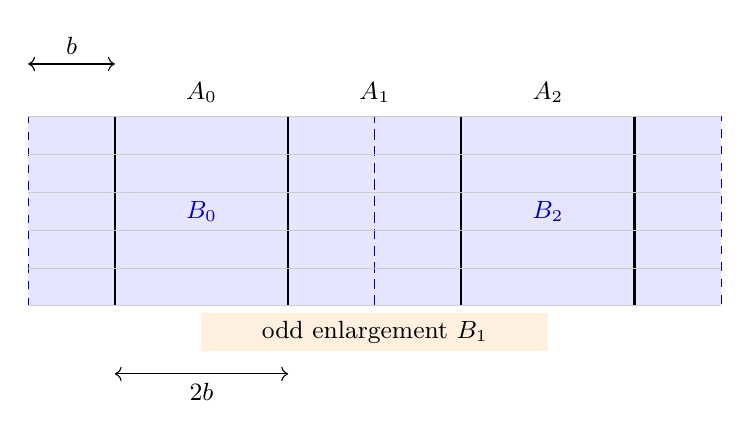
\begin{tikzpicture}[x=0.55cm,y=0.48cm,font=\small]
\fill[blue!10] (-2,0) rectangle (6,5);
\fill[blue!10] (6,0) rectangle (14,5);
\fill[orange!12] (2,-1.2) rectangle (10,-0.2);
\draw[blue!65!black,dashed] (-2,0) rectangle (6,5);
\draw[blue!65!black,dashed] (6,0) rectangle (14,5);
\foreach \x in {0,4,8,12} \draw[thick] (\x,0)--(\x,5);
\foreach \y in {0,1,2,3,4,5} \draw[gray!40] (-2,\y)--(14,\y);
\node at (2,5.65) {$A_0$};\node at (6,5.65) {$A_1$};\node at (10,5.65) {$A_2$};
\node[blue!65!black] at (2,2.5) {$B_0$};\node[blue!65!black] at (10,2.5) {$B_2$};
\node at (6,-0.7) {odd enlargement $B_1$};
\draw[<->] (0,-1.8)--(4,-1.8) node[midway,below] {$2b$};
\draw[<->] (-2,6.4)--(0,6.4) node[midway,above] {$b$};
\end{tikzpicture}
\caption{The even enlarged strips are disjoint; the odd family is shifted. Each family gives a tensor product of narrow-strip states. Opposite-parity localized operators may overlap and need not commute. The construction estimates an overlap of the two states rather than contracting their combined two-dimensional network.}
\label{fig:strips}
\end{figure}

Let $U_{B_j}$ keep only the trajectory's Hamiltonian gates wholly in $B_j$, and the on-site swaps there. Set $V_j=U_{B_j}^\dagger P_jU_{B_j}$. Each $V_j$ is a contraction, and same-parity $V_j$ have disjoint supports. Replacing the $Q_j$ by $V_j$ in \eqref{eq:overlap} costs at most twice the sum of their localization errors, by telescoping products of contractions. No commutation of opposite-parity $V_j$ is asserted.

\subsection{The factorial width--time balance}
Color the bounded-incidence Hamiltonian blocks with at most $kd+1$ colors so that disjoint blocks share a color. The Cayley unitary has an exact Hermitian logarithm supported on its block,
\[
 H_{b,h}^{\rm eff}=\frac2h\arctan(hH_b/2),\qquad
 \nn{H_{b,h}^{\rm eff}}\leq J.
\]
Serializing colors increases physical duration by a fixed factor. In a frame toggled by the swaps, spatial supports and strengths are unchanged. Thus \cref{lem:locality} applies to every sampled history, with constants independent of its number of gates.

Choose $L\geq64$ with $L=O(\log(Q/\xi))$ and $L\geq\log(100m^2/\xi)$. There is a fixed $C_0$, depending on the parameters in \cref{thm:buffer}, such that
\begin{equation}\label{eq:width}
 q=\left\lceil\frac{C_0L}{\log L}\right\rceil,
 \qquad b=a(q+2)
\end{equation}
makes the sum of localization errors at most $\xi/100$. Indeed $CJt\leq C_1\log L$ by \eqref{eq:shorttime}. Stirling's bound $q!\geq(q/e)^q$ gives
\[
 \log\frac{q!}{(CJt)^q}
 \geq q\log\frac q{eC_1\log L}\geq 3L
\]
for sufficiently large fixed $C_0$; the finite interval $64\leq L\leq L_*$ is covered by increasing it once. The factor $e^{CJt}$ and the polynomial support prefactors are absorbed in $L$. In particular,
\begin{equation}\label{eq:balance}
 b(J+\gamma)t=O(L).
\end{equation}

\subsection{Paying for reset registers}
The register count is not bounded by the total number of time steps. In a row of any enlarged strip there are at most $Cb$ physical sites. Its number $N$ of sampled resets is a sum of independent Bernoulli variables of mean at most $Cb\gamma t$. The elementary moment bound
$\E e^N\leq\exp((e-1)Cb\gamma t)$ shows that
\[
 \Prb\{N\geq(e-1)Cb\gamma t+\log(Cm/\eta_h)\}
 \leq\eta_h/(Cm).
\]
There are at most $Cm$ nonempty row segments across the two strip decompositions, including the unused product factors. Choose a deterministic cap above the displayed threshold for each row, and return zero on a history that exceeds a cap. This changes the normalized expectation by at most $\eta_h$. We take $\eta_h=\xi/100$; it is an accuracy budget, independent of confidence $\delta$. We do not require all repeated histories to pass, and do not use a rejection loop.

By \eqref{eq:balance} each good row has $O(L)$ qubits, including passive purification and every retained reset register. Its Hilbert-space dimension is therefore $\exp(O(L))=Q^{O(1)}$.

\subsection{Crossing action controls a constructive compression}
For a vector $\psi$ and a bipartition let $\cN(\psi)$ be the sum of its Schmidt coefficients, equivalently the nuclear norm of its coefficient matrix. A gate wholly on one side preserves this norm. For \eqref{eq:cayley},
\[
 \nn{U_{b,h}-I}\leq Jh.
\]
Expanding the difference into at most $4^k$ Pauli strings gives coefficient one-norm at most $2^kJh$. Each Pauli factors into unitaries on the two sides of any cut. Nuclear-norm submultiplicativity and the triangle inequality give
\begin{equation}\label{eq:nuclear}
 \cN(U_{b,h}\psi)\leq(1+2^kJh)\cN(\psi)
 \leq e^{2^kJh}\cN(\psi).
\end{equation}
This argument remains valid after toggling to different internal registers. Swaps at one spatial site contribute no crossing action. The inserted $P_j$ is a product contraction and does not increase the nuclear norm. Across a horizontal row cut of a strip, only $Cb$ blocks can cross. Consequently every exact intermediate strip vector, including its forward and reversed portions, satisfies
\begin{equation}\label{eq:Bstar}
 \cN(\psi_{\rm exact})\leq B_*:=e^{CbJt}=Q^{O(1)}.
\end{equation}

The following error inequality makes this an algorithmic statement rather than an existence claim about a good matrix-product state.

\begin{lemma}[Compression against an exact reference]\label{lem:compression}
Suppose $\nn\phi\leq1$ and $\cN(\psi)\leq B_*$ across a cut. Remove the tail $r$ beyond the largest $D$ Schmidt coefficients of $\phi$. Then
\begin{equation}\label{eq:compression}
 \nn{\phi-r-\psi}^2\leq\nn{\phi-\psi}^2+\frac{2B_*}{\sqrt{D+1}}.
\end{equation}
After $M_c$ compressions and unitary or contractive local-product updates, total vector error at most $\zeta$ is achieved by a polynomial bond cap, for instance
$D\geq(32M_cB_*/\zeta^2)^2$, with numerical slack.
\end{lemma}
\begin{proof}
Orthogonality of retained and discarded Schmidt pieces gives
\[
 \nn{\phi-r-\psi}^2=\nn{\phi-\psi}^2-\nn r^2+2\Re\ip r\psi.
\]
The operator norm of the discarded coefficient matrix is at most $1/\sqrt{D+1}$. Nuclear/operator-norm duality bounds $|\ip r\psi|$ by $B_*/\sqrt{D+1}$. This proves \eqref{eq:compression}. Each unitary preserves vector error; each product contraction decreases it. Summing the squared-error increments proves the assertion. Finite-precision compressions with constant rank slack obey the same estimate up to paid normwise errors; \cref{app:arithmetic} supplies the construction.
\end{proof}

Group each strip row into one matrix-product site. A whole-block gate has fixed operator bond at most $4^k$; intermediate bond growth is therefore a fixed factor. Its physical row dimension is polynomial, as just proved. There are polynomially many gates and at most a polynomial number $M_c$ of canonical sweeps, chosen before the bond cap. For example, $100(G+1)(m+1)^3$ bounds a procedure that sweeps after every one of $G$ gates. Apply \cref{lem:compression} with $\zeta=\xi/100$. It constructs subnormalized rational matrix-product vectors $\phi_e,\phi_o$ within $\zeta$ of the two localized parity vectors. The complete parity vector is a tensor product over disjoint strips and unused product factors, and can be represented by concatenating their row orderings. The two resulting orderings may differ.

\subsection{A bounded estimator for differently ordered states}
Put $a_x=\bra x\phi_e\rangle$, $b_x=\bra x\phi_o\rangle$ and $Z_0=\nn{\phi_e}^2+\nn{\phi_o}^2\leq2$. If $Z_0=0$ return zero. Otherwise sample
\begin{equation}\label{eq:importance}
 \pi(x)=\frac{|a_x|^2+|b_x|^2}{Z_0},\qquad
 Y(x)=\frac{Z_0\overline{a_x}b_x}{|a_x|^2+|b_x|^2}.
\end{equation}
The zero denominator has sampling probability zero. Directly,
\begin{equation}\label{eq:bounded}
 \E_\pi Y=\ip{\phi_e}{\phi_o},\qquad |Y|\leq Z_0/2\leq1.
\end{equation}
Sample the mixture by choosing one of the two states with weight proportional to its squared norm, then sampling that matrix-product state in its own ordering. Evaluate both amplitudes on the resulting classical string. Each operation is a one-dimensional tensor contraction. A combined two-dimensional tensor network is never contracted.

All tensors are rational after paid approximation. Conditional probabilities and the ratio in \eqref{eq:importance} thus have polynomial bit height; an extremely small nonzero denominator does not imply exponentially many bits. Round categorical distributions to a predetermined dyadic precision with total variation at most $\xi/100$ over all choices. This costs logarithmically many bits per choice in the number of choices and inverse error. The bounded score changes its mean by at most $2\xi/100$.

Finally take the real part and average $O(\xi^{-2}\log(2/\delta))$ independent scores, each using a fresh shared history for its two parity states. Hoeffding's inequality supplies confidence $1-\delta$. Channel error, localization, capped-history bias, vector error, arithmetic and finite-bit sampling fit within $\xi$ after the displayed slack allocations. Every repetition has a deterministic work bound. This completes the proof of \cref{thm:buffer}.

% END sections/buffer

% BEGIN sections/sparse
\section{Sparse propagation with a paid boundary evaluation}\label{sec:sparse}

The buffer theorem evaluates individual product functionals. To use it for a longer interval, we construct a sparse weighted-basis approximation to the later observable. Its error is then smoothed by the earlier interval.

For $A=\sum_\alpha a_\alpha F_\alpha$ write
$\nn a_{\ell_q}=(\sum_\alpha|a_\alpha|^q)^{1/q}$.
This coefficient norm is distinct from the weighted Schatten norm, except at $q=2$.

\begin{lemma}[Finite-step coefficient contraction]\label{lem:coefficient}
There is a fixed $p_c<2$, depending only on $k,d,g$, such that the noisy whole-block updates described below contract $\ell_{p_c}$. They also contract the coefficient two-norm tilted by $e^{\theta W}$, after decreasing the fixed $\theta$ in \cref{lem:weight} if necessary.
\end{lemma}
\begin{proof}
Allocate noise rate $\gamma/(2d)$ to each site of each incident Hamiltonian block, and retain the nonnegative residual one-site rates. Follow a block Cayley conjugation by the Euler maps for its allocated noise. The identity coefficient on that block is fixed. The complementary local coefficient sector is invariant: reference-preserving conjugation fixes identity and is orthogonal in weighted two-norm.

On this active sector the Cayley map has $\ell_2$ norm one and $\ell_1$ norm at most $e^{C_kJh}$. This follows from its local generator norm as in the proof of \cref{lem:weight}; the effective Hamiltonian in the proof of \cref{thm:buffer} has norm at most $J$ and preserves the same reference. Interpolation bounds its $\ell_p$ norm by $e^{C_kJh(2/p-1)}$. Every active coefficient is damped by at least $e^{-\gamma h/(2d)}$ in the subsequent Euler maps. Choose
\[
 s_c=\min\{1/2,\gamma/(4dC_kJ)\},\qquad
 p_c=\frac2{1+s_c},
\]
omitting the second option when $J=0$. The combined active-sector norm is at most one. The identity and active sectors form a direct $\ell_p$ sum. Applying the argument to each fixed outside coefficient proves the global contraction. Residual resets are diagonal contractions.

For the tilted two-norm, the same local row-sum estimate as in \cref{lem:weight} bounds coherent active-sector growth by $e^{C_kJ\sinh(k\theta)h}$. The allocated Euler damping absorbs it when $\theta$ satisfies the displayed smallness bound there. Outside weights multiply all local coordinates by a common factor. Thus the tilted norm also contracts at each finite update.
\end{proof}

This is the coefficient interpolation mechanism of \cite[Lemma~S15 and Corollary~S16]{APTH}, implemented for reference-preserving rational whole blocks. The following truncation estimate is elementary and is also the mechanism of \cite[Lemma~S6]{APTH}.

\begin{lemma}[Constructive sparse approximation]\label{lem:sparse}
Supply the initial observable as an explicit coefficient list, of $\ell_{p_c}$ norm at most $M_p$ and tilted two-norm at most $M_\theta$. Let $Q$ bound that list's description length. On an $m$-site interval with total local action polynomial in $Q$, and $M_p,M_\theta\leq\poly(Q)$, one can construct
\begin{equation}\label{eq:sparse}
 B=\sum_{j=1}^K b_jF_{\alpha_j},\qquad
 \nn{B-\Phi A}_{2,\Sigma_m}\leq\eta,
\end{equation}
in polynomial bit work in the full description, $m$, $\eta^{-1}$ and the stated budgets. Here $K\leq\poly(Q,\eta^{-1})$. If $M_\theta\leq\poly(Q)$ and $\eta^{-1}\leq\poly(Q)$, every retained weight is $O(\log Q)$ and
\begin{equation}\label{eq:paidnorm}
 \sum_j|b_j|\,C_\nu^{|\alpha_j|}\leq\poly(Q)
\end{equation}
for a fixed computable $C_\nu$ bounding $\nn{F_i}_\infty$.
\end{lemma}
\begin{proof}
Discretize segment by segment using \eqref{eq:steps}, with $\xi$ replaced by a fixed fraction of $\eta$. Use the complete noisy blocks of \cref{lem:coefficient}. The weighted two-norm channel error is controlled by the same local telescoping argument: reference-preserving channels are contractions in this norm, and local generator norms are bounded by fixed multiples of $J+\gamma$. Its total number of updates has a known polynomial upper bound $Q_u$.

First consider exact arithmetic. After each complete update, merge equal basis words and discard coefficients below $\tau$. If the coefficient $\ell_{p_c}$ norm is at most $M_p$, then
\begin{equation}\label{eq:threshold}
 \sum_{|a_\alpha|<\tau}|a_\alpha|^2
 \leq\tau^{2-p_c}M_p^{p_c},\qquad
 \#\{|a_\alpha|\geq\tau\}\leq(M_p/\tau)^{p_c}.
\end{equation}
Both coefficient budgets decrease under deletion. Choose a dyadic threshold with
\[
 \tau^{1-p_c/2}M_p^{p_c/2}\leq\eta/(100Q_u).
\]
Because $2-p_c$ is a fixed positive constant, $\tau^{-1}$ is polynomial in the declared budgets. Subsequent two-norm contractions telescope all pruning errors. An update has at most $4^k$ output branches per retained word, so no full coefficient array is enumerated.

For finite arithmetic predeclare doubled budgets $2\max(1,M_p)$ and $2\max(1,M_\theta)$, choose the threshold with these budgets, and choose a polynomial cap $K_{\max}$ larger than the retained-count bound with a factor-two threshold slack. Compute each local update to certified coefficient error $\omega$. Threshold ambiguities can be handled by retaining every coefficient certified to exceed $\tau/2$ and discarding only those certified below $2\tau$; use a deterministic rule in the overlap. This changes only fixed constants in \eqref{eq:threshold}. Impose
\begin{equation}\label{eq:rounding}
 Q_u(4^kK_{\max}+1)\omega
 \leq\frac{\min(\eta,M_p,M_\theta,1)e^{-\theta m}}{10^4}.
\end{equation}
The triangle inequality bounds accumulated $\ell_p$, ordinary two-norm and tilted two-norm rounding errors within their predeclared slack. Thus the cap and threshold are chosen without a circular norm assumption. The required precision has
$O(m+\log Q_u+\log K_{\max}+\log\eta^{-1})$ additional bits. Local basis matrices are computable algebraic functions of rational $p$ of fixed degree; their conversion errors are paid at this precision, enlarged by $O(m\log C_\nu)$ bits. \Cref{app:arithmetic} details the finite operations.

A retained coefficient satisfies
$|b_j|e^{\theta|\alpha_j|}\leq2\max(1,M_\theta)$, while its size is at least a fixed multiple of $\tau$. Therefore $|\alpha_j|=O(\log Q)$ in the claimed regime. Finally $\sum_j|b_j|\leq\sqrt K\nn B_{2,\Sigma_m}$, and $\nn{F_{\alpha_j}}\leq C_\nu^{|\alpha_j|}$ is polynomial. This proves \eqref{eq:paidnorm}.
\end{proof}

The last factor in \eqref{eq:paidnorm} is necessary. The weighted basis consists of Hermitian operators, not of unitaries. Treating each retained word as norm one would omit a polynomial, but consequential, accuracy cost.

\begin{proposition}[Evaluation after an early smoothing interval]\label{prop:smoothingevaluation}
Let $m\leq\poly(\log Q)$ and let the total physical action be $O(\log Q)$. Suppose the initial observable is a specified Hermitian product contraction of support $O(\log Q)$, with polynomial coefficient and tilted budgets. For $\epsilon^{-1}\leq Q$, its specified product-source mean is computable to additive error $\epsilon$ with confidence $1-\delta$ in $\poly(Q,\log(2/\delta))$ work.
\end{proposition}
\begin{proof}
Choose a rational early duration $s=O_\nu(\gamma^{-1}\log(2m))$ for which \cref{lem:HC} reaches $q\geq4m\log(\mu^{-1})$. For example, since $\log(\mu^{-1})\leq\nu^{-1}$, a sufficiently large fixed multiple of $\lceil\log_2(4m/\nu)\rceil/(\nu\gamma)$ works. Then \eqref{eq:normconversion} has factor less than two. If $T<s$, \cref{thm:buffer} evaluates the whole product functional directly. Otherwise expand the original $O(\log Q)$ support in the $F$ basis and apply \cref{lem:sparse} to the \emph{later} interval $[s,T]$, with two-norm error $\eta=\epsilon/100$. The \emph{earlier} channel gives
\[
 \nn{\Phi_{0,s}(\Phi_{s,T}A-B)}_\infty\leq2\eta.
\]
Every word $F_{\alpha_j}$ divided by $C_\nu^{|\alpha_j|}$ is a Hermitian product contraction. Compute the polynomial bound
\[
 S_B=\max\left\{1,\sum_j|b_j|C_\nu^{|\alpha_j|}\right\}.
\]
Use \cref{thm:buffer} to evaluate each normalized functional with error $\epsilon/(100S_B)$. Give each call failure budget $\delta/\max(1,K)$. Here $(J+\gamma)s=O(\log\log Q)$, and the requested buffer inverse precision is polynomial in $Q$. A union bound and \eqref{eq:paidnorm} finish the proof. No channel has been commuted through another interval.
\end{proof}

% END sections/sparse

% BEGIN sections/assembly
\section{Proof of the global-readout theorem}\label{sec:assembly}

We assemble the analytic and computational estimates. All constants in this section depend only on $a,k,d,g,\nu$. It is enough initially to consider
\[
 P=\bigotimes_{i\in S}A_i,\qquad
 A_i=A_i^\dagger,\quad\Tr A_i=0,\quad A_i^2=I,
\]
with identities elsewhere; put $r=|S|$. Identity alone is evaluated exactly.

Let
\begin{equation}\label{eq:Q}
 Q=16+B+n+\lceil\epsilon^{-1}\rceil+\lceil\log_2(2/\delta)\rceil,
 \qquad L=\lceil\log_2 Q\rceil.
\end{equation}
By \cref{lem:entropy}, a rational integer-logarithm test removes all times $\gamma T\geq C_\nu L$: return the known reference mean. Therefore $JT=O_g(L)$ and $\gamma T=O_\nu(L)$ in the remaining branch. Localize with error $\eta=\epsilon/100$ using \cref{lem:locality}. The retained region satisfies
\begin{equation}\label{eq:mr}
 m\leq\min(n,CrL^2).
\end{equation}
The restricted system has the same reference and local estimates.

Put $t_0=2\theta/\gamma$ and $\lambda=\mu\theta$. Choose an early smoothing duration $s$ reaching
\[
 q\geq\max\{2,\,4m\log(\mu^{-1})/(\lambda r)\}.
\]
The lower bound $c_\sigma\geq\nu$ makes a rational choice
\begin{equation}\label{eq:smallS}
 s=O_{\nu,\theta}\!\left(\frac{1+\log(m/r)}\gamma\right)
 =O_{\nu,\theta}(\gamma^{-1}\log L)
\end{equation}
possible by integer logarithm bounds. If $T\geq s+t_0$, apply physical-support damping on the later interval, and then smoothing on the earlier interval:
\begin{equation}\label{eq:largeR}
 \nn{\Phi_{0,T}P}_\infty
 \leq\eta+\mu^{-m/q}e^{-\lambda r}
 \leq\eta+e^{-3\lambda r/4}.
\end{equation}
The first $\eta$ restores the full-system localization error. This order of operations is valid for the prescribed nonautonomous drive.

There are three exhaustive branches.
\begin{enumerate}
\item If $T\geq s+t_0$ and $r\geq C\lambda^{-1}\log(100/\epsilon)$, return zero using \eqref{eq:largeR}.
\item If $T<s+t_0$, evaluate the entire localized evolution by \cref{thm:buffer}. Its region may be global, $m=n$, but \eqref{eq:smallS} gives $(J+\gamma)T=O(\log L)$. The buffer theorem allows precisely this global early-time case.
\item Otherwise $r=O(\log(1/\epsilon))$ and $m=O(L^3)$. Expand $P$ in the $F$ basis on its original support. There are at most $4^r$ terms. Its two-norm is at most one, its coefficient $\ell_{p_c}$ norm is at most $2^r$, and its tilted two-norm is at most $e^{\theta r}$. All are polynomial in $Q$. Apply \cref{prop:smoothingevaluation}.
\end{enumerate}
This proves polynomial prediction for products of traceless Bloch unitaries. The exponent does not hide an extensive support parameter: high support is handled by the first two branches.

\subsection{General Hermitian product factors}
Every one-qubit Hermitian contraction has an ordinary spectral decomposition
\begin{equation}\label{eq:mixture}
 O_i=a_iI+b_iA_i,\qquad
 a_i\in\R,\quad b_i\geq0,\quad |a_i|+b_i\leq1,
\end{equation}
where $A_i$ is a traceless Hermitian unitary if $b_i>0$. Sample independently at site $i$ the signed identity with probability $|a_i|$, $A_i$ with probability $b_i$, and a zero contribution with the remaining probability. Record the product of identity signs. The tensor product is a bounded signed mixture of the products already treated.

The square root in the Bloch length and a normalized axis are handled at certified finite precision. One may approximate each axis by a rational unit vector via one of the two stereographic charts, using the chart whose denominator is bounded away from zero. If $b_i$ is smaller than the local error budget, discard it instead of dividing by it. Compute rational contractions within $O(\epsilon/n)$ per factor; telescoping their tensor product costs $O(\epsilon)$. These operations and categorical sampling have polynomial bit cost. An outer average of $O(\epsilon^{-2}\log(2/\delta))$ bounded estimates, with internal errors and confidence divided over that finite count, proves \eqref{eq:guarantee}. Clip every internal estimate to $[-1,1]$ before averaging. This completes the proof of \cref{thm:main}.

\begin{remark}[The correct mixture is unweighted]
Equation~\eqref{eq:mixture} uses the ordinary Bloch decomposition. Replacing $a_i$ by $\Tr(\sigma O_i)$ would not generally preserve $|a_i|+\nn{O_i-a_iI}\leq1$. Weighted centering is useful for the coefficient estimates, but not for this bounded sampling representation.
\end{remark}

\subsection{Complete resource closure}
The late-time test is made before numerical evolution, so an exponentially large rational horizon or rate incurs its binary input cost, not an unbounded numerical action. In every nontrivial branch the total local action is $O(nL)$ on at most $n$ sites, and $O(L^4)$ in the sparse region. \eqref{eq:totalsteps} gives polynomial gate counts including every supplied control segment. The threshold exponent depends only on $p_c<2$; all retained coefficient counts, their paid one-norms and inverse buffer errors are polynomial. In the buffer,
\[
 \log q_{\rm row}=O(\log Q),\qquad
 \log B_*=O(\log Q),\qquad
 \log D=O(\log Q+\log M_c+\log\xi^{-1}).
\]
Every dense matrix consequently has polynomial dimension. Certified arithmetic requires polynomially many precision bits, including the algebraic weighted basis and source square roots. Finite random choices have a bounded total count and a paid total-variation error. Confidence occurs only in repetition counts and their logarithmic sub-budgets. These estimates establish bit complexity and deterministic work bounds on all runs; they do not assert that the polynomial degrees are small.

% END sections/assembly

% BEGIN sections/sampling
\section{When the same ingredients give a full-output sampler}\label{sec:sampling}

A scalar expectation algorithm need not supply a positive joint distribution. A supplied interaction tree with small crossing action does supply enough additional structure. We state the result separately because a general square lattice does not have this property.

A binary leaf tree has the physical sites as its leaves and internal degree at most three. Removing an edge $e$ partitions the leaves into $A_e,B_e$. A tree-tensor vector is a contraction of tensors on this acyclic graph; its virtual bond on edge $e$ bounds the Schmidt rank across that partition. Its norm, amplitudes and sequential local-outcome probabilities are computable by contractions on the tree. These are the standard operations of \cite[Theorems~1--4]{SDV}; see also \cite[Sections~2.2 and~3.2]{Seitz}.

\begin{theorem}[Supplied bounded-cut sampler]\label{thm:cuts}
Fix $k,d,c,r_0,g,\nu$. Supply a binary leaf tree, a normalized rational tree-tensor purification of the input with local space $\C^2\otimes\C^{r_0}$ and bond dimension at most $D_0$, and a finite rational Hamiltonian schedule. Suppose each block has at most $k$ sites, norm at most $J$, incidence at most $d$, preserves the full-rank product reference $\Sigma$, and at most $c$ active blocks cross any tree edge in any segment. Evolve with \eqref{eq:model}, $J/\gamma\leq g$, $\mu\geq\nu$.

For a supplied terminal product POVM with a fixed bounded number of rational effects per site, there is a bounded-work classical sampler whose law is within $\epsilon$ in total variation of the physical outcome law. Its bit work is polynomial in the complete input length, $n,D_0,\epsilon^{-1}$. No spatial embedding is required for this theorem. The cut certificate is supplied and can be checked directly.
\end{theorem}
\begin{proof}
The entropy estimate \eqref{eq:entropy} applies also to the correlated supplied input. For $\gamma T\geq C_\nu\log(n/\epsilon)$ sample the product reference POVM law. Otherwise $JT=O_{g,\nu}(\log(n/\epsilon))$.

Discretize by \eqref{eq:cayley}--\eqref{eq:steps}, paying channel error $\epsilon/100$. The total number $G$ of gates and reset choices is polynomial in the explicit schedule, $n$ and $\epsilon^{-1}$. Represent each reset by a swap with a sampled local ancillary register, keeping the old register at that leaf. The number of resets at one leaf has mean at most $\gamma T$. The exponential-moment estimate used above gives a simultaneous cap
\[
 C[\gamma T+\log(n/\epsilon)]=O_\nu(\log(n/\epsilon))
\]
except on histories of probability at most $\epsilon/100$. On a failed history output a sample from any fixed product law. This modifies total variation by at most $\epsilon/100$ and keeps work bounded. Good histories have polynomial local leaf dimension.

Initially $\cN_e(\Psi_0)\leq\sqrt{D_0}$. For a crossing whole-block gate, \eqref{eq:nuclear} applies across the leaf partition. Noncrossing gates and on-leaf swaps preserve that nuclear norm. At every exact intermediate step,
\begin{equation}\label{eq:treeaction}
 \cN_e(\psi_{\rm exact})\leq
 B_*:=\sqrt{D_0}\exp(2^kcJT).
\end{equation}
This is polynomial after the entropy cutoff. A fixed-support gate has a tree-operator representation of bond at most $4^k$: expand it in product Paulis and carry the common summation index along its support's Steiner tree. Apply the gate, then make a canonical sweep through the edges and compress there. Canonical subtrees identify each edge's Schmidt decomposition with an SVD of a local matrix; no full coefficient matrix is constructed. Intermediate bond growth is a fixed factor.

Choose a polynomial upper bound $M_c$ on all gate sweeps and set
$D\geq(128M_c B_*/\epsilon^2)^2$, with constant rank slack. \Cref{lem:compression} and the gap-free arithmetic construction in \cref{app:arithmetic} give a subnormalized rational tree vector $\phi$ within $\epsilon/100$ of the exact unit history vector. If $\psi$ is unit and $\nn{\psi-\phi}\leq\zeta$, normalization of $\phi$ changes it by at most $\zeta$; the corresponding pure density matrices are within $4\zeta$ in trace norm. Partial trace and the final POVM contract this distance. Thus the conditional outcome law is within $2\zeta$ in total variation, uniformly in every good history.

For a product POVM, each conditional weight is a rational tree contraction of the chosen effects and identities. It is nonnegative. Sequential sampling needs no square root of an effect and no lower bound on a nonzero outcome probability. The normalization cancels from the conditional ratios. Their bit height is polynomial. Round each categorical distribution so that the sum of its TV errors is at most $\epsilon/100$, and do the same for the reset choices. Averaging histories, and adding discretization and capped-history errors, proves the theorem.
\end{proof}

The more general parameter exposed by the proof is crossing action:
\[
 \max_e\sum_jt_j\sum_{b\text{ crosses }e}\nn{H_{b,j}}.
\]
Without a noise cutoff the same constructive simulation costs a polynomial in the explicit description, total generator action, inverse error, and the exponential of this crossing action. Noise makes the latter polynomial on bounded cuts.

Chains, fixed-width ladders and suitable bounded-degree trees admit fixed $c$. A full $L\times L$ interaction grid has a balanced separator with $\Omega(L)$ crossing nearest-neighbor edges. Any binary leaf tree has a balanced edge, so no constant-$c$ certificate exists for the full grid. The bound here is then exponential in $LJT$. This is a limitation of this proof, not a sampling lower bound.

\subsection{A stronger late-time certificate}
The reference sampler is particularly accurate after logarithmic time. This follows directly from known hypercontractivity and a Hilbert--Schmidt gap; it is not a separate simulation mechanism.

\begin{proposition}[Relative mixing for unbiased resets]\label{prop:relative}
For $\sigma=I/2$, arbitrary initial states and arbitrary bounded time-dependent Hamiltonians, without a locality restriction,
\begin{equation}\label{eq:relative}
 \nn{2^n\rho_T-I}_\infty\leq4ne^{-\gamma T}
 \quad\text{if }\gamma T\geq\log n.
\end{equation}
In particular, $\gamma T\geq\log(4n/\eta)$ implies
$(1-\eta)I/2^n\leq\rho_T\leq(1+\eta)I/2^n$.
\end{proposition}
\begin{proof}
King's Corollary~2, interleaved with the actual unitary conjugations, gives normalized Schatten $p$-to-$q$ contraction when $q-1\leq e^{2\gamma t}(p-1)$. It applies to Schr\"odinger propagation as well, since the unbiased reset is self-adjoint. Put $R=2^n\rho$ and $a=\log n/(2\gamma)$. At $p=1+1/n$, $\nn{R_0}_{p,I/2^n}\leq2^{n/(n+1)}<2$. After time $a$, hypercontractivity to exponent two gives
$\nn{R_a-I}_{2,I/2^n}^2<3$.
Every centered operator contracts in two-norm at rate $\gamma$: the Hamiltonian is skew and every nonidentity Pauli coefficient is damped at least that fast. Evolve for $T-2a$. A last interval of length $a$ is two-to-$(n+1)$ hypercontractive, and $\nn X_\infty\leq2^{n/(n+1)}\nn X_{n+1,I/2^n}<2\nn X_{n+1,I/2^n}$. Hence the bound is at most $2\sqrt3 e^{-\gamma(T-2a)}\leq4ne^{-\gamma T}$. For $n=1$, take $a=0$.
\end{proof}

The operator inequality controls every positive effect simultaneously. In particular it gives relative accuracy for all computational-basis marginals, including exponentially small ones, by using their uniform reference probabilities. It does not give this operation before its stated mixing time.

\subsection{A small nonlocal output law}
\begin{corollary}[Logarithmically many parity checks]\label{cor:syndrome}
Under the unbiased case of \cref{thm:main}, let $r\leq C\log Q$ commuting Pauli observables be supplied, with $C$ fixed. Their joint projective measurement law has a classical TV-$\epsilon$ sampler in polynomial work, and can be tabulated to that accuracy. The Pauli strings may be nonlocal.
\end{corollary}
\begin{proof}
For $S\subseteq[r]$, the product of the commuting observables is a signed Hermitian Pauli string, whose mean $m_S$ is predicted by \cref{thm:main}. Walsh inversion gives
$p(x)=2^{-r}\sum_S(-1)^{x\cdot1_S}m_S$.
Estimate all $2^r$ moments to error at most $\epsilon/(100\,2^r)$ with divided confidence. The resulting table has total $\ell_1$ error at most $\epsilon/100$. Clip its negative entries and normalize; this increases the error by at most a fixed factor. Finite-bit sampling adds a paid TV error. Allocate the moment-computation failure probability as another TV budget. All counts and inverse accuracies are polynomial when $r=O(\log Q)$.
\end{proof}

% END sections/sampling

% BEGIN sections/acquisition
\section{Acquisition and controlled reuse}\label{sec:acquisition}

The main algorithm assumes that the local generator is given. We now show what can be acquired once and reused for new experiments. This section uses unbiased replacement, known $\gamma$, a fixed local Pauli dictionary, calibrated preparation and readout contrast, and prescribed coherent controls. The learning and rapid-mixing stability principles have established predecessors \cite{MBFR,LCMP}; the additional operation is a polynomial evaluator for each later query.

Let the unknown static drift be
$H_0=\sum_{P\in\mathcal D}h_PP$, with $M_{\rm par}=|\mathcal D|$, $|h_P|\leq J_0$. The dictionary has bounded range, support and incidence and includes no duplicate nonidentity strings. Future controls $H_c(t)$ are known rational schedules such that $H_0+H_c(t)$ has the fixed local bounds. Choose fixed bounds also for the drift dictionary and control dictionary separately; the clipped learned table then satisfies these bounds, and their union enlarges the simulation constants by at most a fixed factor. The controls involve no intervening measurements, fresh physical registers or unspecified cooling. An empty unknown dictionary needs no acquisition.

\subsection{Two stability scales}
For a bounded-support $O$, locality and mixing combine to give a relaxation bound independent of total volume. Specifically \eqref{eq:LR} with radius $R(x)=\lceil r_0+r_1x\rceil$, $x=\gamma(t-s)$, and sufficiently large fixed $r_0,r_1$, has error at most $e^{-2x}$. Its restricted region has $O((1+x)^2)$ sites. Apply \eqref{eq:entropy} there for every reduced input state and use duality. For an explicit fixed $A$,
\begin{equation}\label{eq:localrelax}
 \nn{\Phi_{s,t}O-\tau(O)I}
 \leq\min\{2,A(1+x)e^{-x/2}\},\qquad
 \tau(O)=2^{-n}\Tr O.
\end{equation}
The constants depend on the support bound, local geometry and $g$, not on volume, horizon or the number of switches.

\begin{proposition}[Local and global perturbation budgets]\label{prop:stability}
Let the actual Heisenberg generator differ from the unbiased reference by local maps $B_{z,t}$ with $B_{z,t}(I)=0$, norm at most $\eta$, bounded support radius and bounded density. Assume only that the total actual Schr\"odinger evolution is CPTP. Then, for each fixed-local $O$ of norm at most one,
\begin{equation}\label{eq:localstable}
 \sup_{s\leq t}\nn{\Phi'_{s,t}O-\Phi_{s,t}O}
 \leq K_{\rm st}\eta/\gamma.
\end{equation}
The actual evolution need not preserve the maximally mixed state. For a general $\nn O\leq1$, if there are $M$ perturbation terms,
\begin{equation}\label{eq:globalstable}
 \sup_{s\leq t}\nn{\Phi'_{s,t}O-\Phi_{s,t}O}
 \leq\frac{M\eta}{\gamma}[4\log(2n)+4].
\end{equation}
For product sources whose one-site trace-norm differences are at most $\zeta$, the fixed-local mean changes by at most $K_{\rm pr}\zeta$, uniformly in horizon and volume. No assertion about arbitrary correlated sources follows from their one-site marginals.
\end{proposition}
\begin{proof}
Duhamel's formula places the reference future propagator next to $B_{z,u}$ and the actual propagator outside. The latter is a norm contraction. Near the future support, within $R(x)$ plus the perturbation radius, there are at most $C(1+x)^2$ terms. Since they annihilate identity, \eqref{eq:localrelax} bounds their contribution by
$\eta C A(1+x)^3e^{-x/2}$.
For a farther term at distance $r$, restrict the observable to a neighborhood disjoint from that term. The term annihilates the restriction. \eqref{eq:LR}, and the square-lattice shell bound $C(r+1)$, give a summed far contribution at most $\eta C'(1+x)e^{-2x}$ after increasing $r_0,r_1$. Integration over physical time gives \eqref{eq:localstable}, for example with
$K_{\rm st}=158CA+C'$, because
$\int_0^\infty(1+x)^3e^{-x/2}dx=158$ and
$\int_0^\infty(1+x)e^{-2x}dx=3/4$.
All constants are obtained from the displayed locality constants by finite geometric sums. This is the near/far rapid-mixing argument of \cite[Theorem~1]{LCMP}, with the proof above making its nonautonomous application explicit.

For global $O$, duality in \eqref{eq:entropy} gives
$\nn{\Phi_{s,t}O-\tau(O)I}\leq\min(2,\sqrt{2n\log2}\,e^{-x/2})$.
Sum the $M$ norms and integrate, splitting at $x=2\log(2n)$, to obtain \eqref{eq:globalstable}. The integral is bounded by $4\log(2n)+4$.

For product sources telescope one factor at a time. Each difference has zero trace and hence annihilates identity. Apply the same near/far estimates to the corresponding single-site functional, now without a time integral. The suprema of the displayed decaying polynomial functions are finite, giving computable $K_{\rm pr}$. This proof requires the telescoping product structure.
\end{proof}

\subsection{An explicit noisy acquisition protocol}
For each $P\in\mathcal D$, choose a one-site Pauli $Q$ anticommuting with $P$ and put $R=iPQ$, including its sign. Pauli orthogonality gives
\begin{equation}\label{eq:learnidentity}
 \tau(R\cG Q)=2h_P,\qquad\tau(RQ)=0.
\end{equation}
The replacement contribution is orthogonal to $R$.

For each shot choose independent uniform signs $s_i$ on $\supp R$. Prepare there $(I+s_ip_iR_i)/2$, with known $p_i\geq p_0>0$; prepare $I/2$ elsewhere, for instance by independently mixing opposite noisy preparations. Measure $Q$ after a short evolution with controls off. The binary outcome $Y$ has a calibrated affine mean $b_Q+c_Q\langle Q\rangle$, where $c_Q\geq c_0>0$ is known. Signed averaging of the corrected score gives
\begin{equation}\label{eq:score}
 |Z|\leq A_{\rm ac}:=\frac2{c_0p_0^k},\qquad
 \E Z(t)=\tau(R\Phi_{0,t}Q).
\end{equation}
Indeed the product-sign average of the prepared state is $(\prod_i p_i)R/2^n$; the calibrated division removes this factor. No entangled probe or inverse evolution is required.

Put $\Gamma=2dJ_0+2\gamma$ and $C_2=k\Gamma^2$. The local generator expansion gives $\nn{\cG^2Q}\leq C_2$: the terms in $\cG Q$ have total norm at most $\Gamma$ and support at most $k$, and the next application costs at most $k\Gamma$. The contraction Taylor formula therefore implies
\begin{equation}\label{eq:learnbias}
 \abs{\frac{\E Z(t)}{2t}-h_P}\leq C_2t/4.
\end{equation}
For target coefficient accuracy $0<\alpha\leq1$ choose the exact rational time
\begin{equation}\label{eq:learntime}
 t=\min\{1/(4\Gamma),\alpha/(4C_2)\}
\end{equation}
and at least
\begin{equation}\label{eq:shots}
 N_P=\left\lceil\frac{8A_{\rm ac}^2}{t^2\alpha^2}
 \log\frac{2M_{\rm par}}{\delta_{\rm ac}}\right\rceil
\end{equation}
shots per coefficient. Hoeffding and a union bound, rounding by at most $\alpha/8$ and clipping to $[-J_0,J_0]$, give simultaneous coefficient error at most $\alpha$, with the slack below. The sample exponent is deliberately conservative, $O(\alpha^{-4})$ at fixed rates. More efficient local learning is available under its own access hypotheses \cite[Theorem~4.9]{MBFR}; we make no optimality claim for \eqref{eq:shots}.

Calibration is a resource assumption. A systematic corrected-mean error $\beta$ contributes $\beta/(2t)$, and timing error $\Delta t$ contributes at most $\Gamma\Delta t/(2t)$. Requiring $\beta\leq\alpha t/8$ and $\Gamma\Delta t\leq\alpha t/8$ fits the slack in the coefficient bound. Add the actual cost $C_{\rm cal}(\beta,\delta_{\rm cal})$ of trusted calibration, or retain these terms as error floors. Repetition cannot remove an unknown fixed bias. Unknown preparation and measurement maps do not acquire identifiability merely from the equations above.

\subsection{A paid finite-rate preparation interface}
The product preparation in \eqref{eq:score} can be approximated even while the unknown drift remains on, at an explicit control cost. Suppose a calibrated local primitive swaps a site with a fresh ancilla in its chosen known full-rank state $\omega_i$ at Poisson rate $\kappa$. Such a state can be a fixed-temperature Gibbs qubit, rotated to the selected axis; its polarization and control accuracy are part of the primitive, not inferred from a bath label. Let $\omega=\bigotimes_i\omega_i$. Reset-only evolution for time $\tau_p$ differs from $\omega$ by at most $2ne^{-\kappa\tau_p}$ in trace norm from any initial state: couple to the event that every site has reset at least once. The always-on drift and noise have total diamond norm at most $n\Gamma$, so Duhamel gives
\begin{equation}\label{eq:physicalprep}
 \nn{\rho_{\rm prep}-\omega}_1
 \leq2ne^{-\kappa\tau_p}+n\Gamma\tau_p.
\end{equation}
For target $b$, take
\[
 L_p=\lceil\log_2(16n/b)\rceil,\qquad
 \tau_p=b/(4n\Gamma),\qquad \kappa=L_p/\tau_p.
\]
Then \eqref{eq:physicalprep} is less than $b/2$. Choosing $b\leq\alpha t/(16A_{\rm ac})$ fits the acquisition bias budget. This requires finite but polynomially growing reset strength and instantaneous ancilla flux. It is not a fixed-hardware preparation theorem. There are $nL_p$ expected swaps and consumed ancillas per shot; a Poisson tail gives a finite high-confidence cap, whose failure is paid in $\beta$ or the confidence budget. Unknown ancilla errors create a declared calibration floor.

\begin{theorem}[An acquired predictor for new interventions]\label{thm:service}
Under the access conditions above, acquire the drift table once at simultaneous coefficient accuracy $\alpha$. Store the rational coefficients, dictionary, noise rate, uncertainty and calibration record, and a spatial index. For each later query supply a product source, an allowed new coherent drive, a global Hermitian product contraction, a binary horizon and numerical error/confidence. A polynomial-work evaluator returns $\widehat f_j$ satisfying, on the acquired-coefficient event,
\begin{align}\label{eq:service}
 \abs{\widehat f_j-f_{{\rm actual},j}}
 \leq{}&\epsilon_{{\rm num},j}+b_{\rm source}+b_{\rm read}\notag\\
 &+\frac{4\log(2n)+4}{\gamma}
       (2M_{\rm par}\alpha+M_{\rm miss}b_{\rm miss}),
\end{align}
except with the declared numerical failure probability. Here the actual dynamics may have $M_{\rm miss}$ additional local difference maps of norm at most $b_{\rm miss}$, the total actual evolution must be CPTP, $b_{\rm source}$ is a global trace-norm source error, and $b_{\rm read}$ is an operator-norm readout error. For fixed-local queries these terms can instead be bounded by
\begin{equation}\label{eq:localservice}
 \epsilon_{{\rm num},j}+K_{\rm st}(2\alpha+b_{\rm miss})/\gamma
       +K_{\rm pr}\zeta+b_{\rm read},
\end{equation}
when the discrepancy density is fixed and source errors are independent products of one-site error at most $\zeta$.
\end{theorem}
\begin{proof}
The learned Hamiltonian satisfies the same locality promises after coefficient clipping. \Cref{thm:main} evaluates each proposed query. A coefficient discrepancy produces the local map $i[(h_P-\widehat h_P)P,\cdot]$, of norm at most $2\alpha$. Apply \cref{prop:stability} and then the trace-norm source and operator-norm readout bounds to obtain \eqref{eq:service}. Its local variant is \eqref{eq:localservice}.

The coefficient-validity event is uniform over every allowed future control, so no union over controls is needed. Assign numerical failures summably, for example $\delta_j=6\delta_{\rm num}/(\pi^2j^2)$. Conditioning on earlier answers still leaves the next algorithmic guarantee valid for the chosen query. All countably many, possibly adaptively selected queries then satisfy their bounds except with probability $\delta_{\rm ac}+\delta_{\rm cal}+\delta_{\rm num}$ and any declared preparation failure.
\end{proof}

For global precision $\epsilon$, taking $\alpha=O(\gamma\epsilon/[M_{\rm par}\log(2n)])$ keeps acquisition operation counts and storage polynomial. Independent one-site source errors can be summed for $b_{\rm source}$; local factor readout errors telescope for $b_{\rm read}$. There are $M_{\rm par}N_P$ shots, at most $n$ local preparations and one local readout per shot, interrogation time $t$ per shot, preparation time $\tau_p$ per shot, and the stated reset flux and calibration costs. The stored table uses $O(M_{\rm par}\log(1/\alpha))$ coefficient bits beyond the input-height and calibration records. Physical duration retains its actual inverse-rate scaling, including $1/\gamma$; polynomial arithmetic in the bits of a small rate does not make that duration free. The predictor performs no future target experiment and solves no full many-body state. It is confined to the specified Markovian, replacement-noise, product-source and coherent-control class.

% END sections/acquisition

% BEGIN sections/obstructions
\section{Two limits of scalar prediction}\label{sec:obstructions}

Additive product-readout prediction is an extensive family of tasks. It is nevertheless weaker than a relative probability evaluator or a positive description of an entire distribution. The following results make those separations precise.

\subsection{Rare probabilities at positive noise}
\begin{theorem}[Relative and logarithmic evaluation]\label{thm:rare}
Fix any positive rational $\gamma$, and set the interaction bound $J=1$. On finite square-lattice regions, with static commuting weight-three Pauli Hamiltonians of range one and site incidence at most twelve, a randomized evaluator of a specified computational-basis outcome probability to relative error $1/2$, or of its logarithm to additive error $1/4$, at every positive rational time, with success probability at least $3/4$ and polynomial complete binary input work, would imply $\mathsf{NP}=\mathsf{RP}$. The input is the pure product $\ket{0^n}$, every site has maximally mixed replacement at rate $\gamma$, and all probabilities in the reduction are strictly positive with logarithm magnitude $O_\gamma(n^2)$.
\end{theorem}
\begin{proof}
Moore and Robson prove NP-completeness of tiling explicit finite square-lattice regions by rotated right trominoes \cite[Sections~3 and~3.1]{MR}. Holes are allowed. This is their unnumbered decision result, not a counting-completeness assertion. A right tromino occupies three cells of a unit square. Let $R$ be such a region, $n=3m$, and let $q_R$ count its tilings. Enumerate all allowed tromino placements $S\subset R$ and set
\begin{equation}\label{eq:tilingH}
 H_R=\sum_S X_S,\qquad X_S=\prod_{i\in S}X_i.
\end{equation}
Each site is in at most four unit squares and at most three placements in each square, giving incidence twelve. The blocks commute and have norm one. There are $M\leq4n$ of them. Placements with a missing lower-left corner are included; enumeration ranges over all possible unit-square anchors, not only sites of $R$.

Consider the target probability $p_R(t)$ of $1^n$ from $0^n$ under the actual Lindbladian. The noise identity is
\[
 \gamma(\reset_i-\Id)=\frac\gamma4\sum_{P=X,Y,Z}(\operatorname{Ad}_{P_i}-\Id).
\]
In a computational matrix unit $\ket a\bra b$, a Hamiltonian left or right multiplication flips three coordinates on one side. A noise conjugation flips at most two coordinates in total, one ket and one bra. To reach $\ket{1^n}\bra{1^n}$ from $\ket{0^n}\bra{0^n}$ requires at least $2n$ flips. Thus every Taylor coefficient below degree $r=2n/3=2m$ vanishes. At degree $r$, every factor must be Hamiltonian and every differing coordinate must flip once. The factors on each side form a disjoint tromino cover. Each cover has $m!$ orderings, canceled by the exponential denominator, and every ket cover has phase $(-i)^m$. Therefore, exactly,
\begin{equation}\label{eq:leading}
 p_R(t)=q_R^2t^r+\mathcal E_R(t).
\end{equation}
This excludes noise at leading order within the density-matrix generator; it does not commute the dissipative channel through $H_R$.

Let $C=\max(1,\lceil2M+2\gamma n\rceil)$, which bounds the induced trace-norm generator norm. For $0<t\leq1$, the full Taylor tail satisfies
\[
 |\mathcal E_R(t)|\leq e^C t^{r+1}.
\]
Choose $T_R=2^{-(2C+20)}$. Since $e/4<1$,
\begin{equation}\label{eq:separation}
 q_R=0\Longrightarrow p_R(T_R)\leq2^{-20}T_R^r,
 \qquad
 q_R\geq1\Longrightarrow p_R(T_R)\geq(1-2^{-20})T_R^r.
\end{equation}
The time has $O_\gamma(n)$ binary digits, and $T_R^r$ has $O_\gamma(n^2)$ digits. All other data are polynomially explicit. A logarithmic estimate with error $1/4$, compared to $r\log T_R-1$, or a relative estimate with error $1/2$, separates the cases with a constant gap.

These probabilities are positive even when no tiling exists. In the Poisson Pauli unraveling, consider histories with exactly one $X$ jump at each site and no other jumps. They have total weight
$w=e^{-3\gamma nT_R/4}(\gamma T_R/4)^n>0$.
All their jumps commute with $H_R$. The conditional target probability is
$|\bra{0^n}e^{-iT_RH_R}\ket{0^n}|^2\geq(1-MT_R)^2$.
Thus $p_R(T_R)\geq w(1-MT_R)^2>0$, and $-\log p_R(T_R)=O_\gamma(n^2)$.

The hypothetical evaluator gives a bounded-error polynomial decision algorithm for the NP-complete tiling problem and hence for SAT. Amplify its decision success, use the standard SAT self-reduction to find an assignment, and verify that assignment. Unsatisfiable formulas are never accepted after verification; satisfiable ones yield a valid witness with probability bounded away from zero. Therefore SAT is in RP and $\mathsf{NP}=\mathsf{RP}$.
\end{proof}

The same instances are exponentially close to a trivial sampler:
\begin{equation}\label{eq:trivialsampler}
 \TV(P_{T_R},\delta_{0^n})\leq\tfrac12(e^{CT_R}-1).
\end{equation}
Consequently \cref{thm:rare} is not a TV-sampling obstruction. It uses exponentially small numerical times with polynomial binary descriptions; it does not establish hardness at a fixed lower time or with exclusively two-body interactions. Padding the region to a polynomial-size rectangle by decoupled noisy sites preserves the reduction, after multiplying by their known product output probability.

\begin{corollary}[The conservation condition does not remove the obstruction]\label{cor:dualrail}
For every fixed full-rank rational $\sigma$ and positive rational $\gamma$, the implication in \cref{thm:rare} also holds in the reference-preserving biased class, with support size six, range three and incidence twelve.
\end{corollary}
\begin{proof}
Replace logical site $i=(x,y)$ by physical sites $(2x,y)$ and $(2x+1,y)$. Put
$E_i=(X_{i,a}X_{i,b}+Y_{i,a}Y_{i,b})/2$.
It has norm one, exchanges $\ket{10}$ and $\ket{01}$, vanishes on $\ket{00},\ket{11}$, and commutes with $\sigma\otimes\sigma$. For each tromino use the whole block $K_S=\prod_{i\in S}E_i$. Start in $\ket{10}^{\otimes n}$ and target $\ket{01}^{\otimes n}$.

There are $4n$ differing ket/bra coordinates. A Hamiltonian multiplication flips six and a one-site biased reset changes at most two, or kills the matrix unit. Hence degree below $2n/3$ vanishes and the leading coefficient is again $q_R^2$. The same norm and Taylor-tail proof applies with $N=2n$ physical sites. Strict positivity follows from the history with exactly one reset per physical site, each to its target bit. Its weight is at least $e^{-\gamma NT}(\gamma T\mu)^N$. Without Hamiltonian its output is exactly the target; with the fixed reset history, contractive telescoping changes it by at most $2MT<1$. This gives a positive lower bound with polynomial logarithm. All block, range and reference promises are satisfied.
\end{proof}

\subsection{All product means can miss almost all of a law}
The next obstruction is information-theoretic and concerns the contract of a mean oracle. It does not give hardness for a generator whose full description is available.

\begin{theorem}[Product-mean indistinguishability]\label{thm:code}
For any fixed $0<\kappa<1$, there exist explicit finite probability laws $P_n$ on $\{0,1\}^n$, each obtained by independently flipping the coordinates of a uniformly random binary linear-code word, such that
\begin{equation}\label{eq:codeTV}
 \TV(P_n,U_n)\longrightarrow1,
\end{equation}
while their diagonal quantum states satisfy, for some fixed $c>0$,
\begin{equation}\label{eq:codemeans}
 \sup_{\substack{O=\bigotimes_iO_i\;\text{Hermitian}\\\nn{O_i}\leq1}}
 \abs{\Tr[O(\rho_{P_n}-I/2^n)]}\leq e^{-cn}.
\end{equation}
Thus even uniform exponentially small errors on all bounded Hermitian product means do not in general provide a total-variation description.
\end{theorem}
\begin{proof}
Let $q=(1-\kappa)/2$ and write $h_2$ for binary entropy. Choose $0<R<1-h_2(q)$ and then $\delta_*>0$ with $h_2(\delta_*)<R$. Random rate-$R$ binary linear codes have dual minimum distance at least $\delta_*n$ with positive probability for all large $n$: the expected number of nonzero dual words of weight at most $\delta_*n$ is at most $2^{n(h_2(\delta_*)-R)+o(n)}$. Fix one such code $C_n$. A finite exhaustive search is one explicit specification; no efficient code-discovery theorem is needed here.

Let $X=C+Z$, with $C$ uniform on $C_n$ and $Z$ independent Bernoulli-$q$ bits. For any coordinate set $S$,
\begin{equation}\label{eq:codefourier}
 \E(-1)^{\sum_{i\in S}X_i}
 =1_{\{1_S\in C_n^\perp\}}\,\kappa^{|S|}.
\end{equation}
All nonconstant Fourier moments of weight below $\delta_*n$ vanish. For a diagonal state only the diagonal part of $O_i$ contributes. Write that part $a_iI+b_iZ$; Hermitian contraction gives $|a_i|+|b_i|\leq1$. Expanding the product and using \eqref{eq:codefourier} bounds its difference from uniform by
\[
 \kappa^{\delta_*n}\sum_{S\subseteq[n]}
       \prod_{i\notin S}|a_i|\prod_{i\in S}|b_i|
 \leq\kappa^{\delta_*n}.
\]
This proves \eqref{eq:codemeans} with $c=\delta_*\log(\kappa^{-1})$.

Choose $s>0$ with $R+h_2(q+s)<1$. With probability tending to one, $X$ lies in the union of Hamming balls of radius $(q+s)n$ around the codewords. That set has size at most $2^{n(R+h_2(q+s))+o(n)}$, so its uniform probability tends to zero. This proves \eqref{eq:codeTV}.
\end{proof}

Given a generator matrix the laws in \cref{thm:code} are easy to sample: sample a message and the independent flips. The theorem is therefore not a complexity lower bound. It shows that a black-box additive mean contract cannot alone justify a full sampler. The family has correlated preparations, not the single product preparation of \cref{thm:main}. At unbiased reset time $t$ it can also be viewed as a code mixture with $\kappa=e^{-\gamma t}$ and $H=0$; the obstruction remains a statement about retained scalar information, not a difficult Hamiltonian.

% END sections/obstructions

% BEGIN sections/discussion
\section{Scope and remaining problems}

The main theorem earns specified-input prediction of nonlocal product readouts at every fixed positive replacement-noise ratio in two dimensions. Its reference-preserving biased extension includes strongly interacting exchange and diagonal models, but it is not a theorem about arbitrary physical cooling. The faithful product reference, conservation, source representation and explicit control schedule are all substantive. In particular, no inference about a generic interacting Gibbs state, a non-Markovian environment, arbitrary measurement feedback or fault-tolerant processing follows.

The mechanism has two complementary representations. Coefficient space compresses the later Heisenberg observable; a positive enlarged-trajectory representation evaluates its earlier boundary functional. A small two-norm error becomes useful only after its functional is actually controlled and constructed. The reset-register construction extends that bridge beyond random-unitary noise without requiring exponentially accurate approximation of an ideal many-body evolution. The resulting polynomial degrees can be extremely large. This is a complexity theorem, not an implemented general-purpose simulator or a hardware-cost advantage.

The most immediate unresolved operation is full-output sampling on a general two-dimensional interaction graph before the logarithmic mixing time. The bounded-cut sampler and late operator-order certificate handle two genuine regimes. The rare-probability reduction does not obstruct TV sampling, and the noisy-code example does not obstruct a method that uses the complete local generator. A positive, locally consistent representation in physical time could therefore be stronger than either of the scalar representations used here. A direct substitution into a fixed-per-layer-noise circuit theorem does not settle that construction.

Two other boundaries deserve separate treatment. First, the conservation condition may be relaxed perturbatively, but the stability argument gives an explicit accuracy floor, not arbitrary-precision simulation of all nonunital dynamics. Second, the product-source condition can be replaced by specified efficiently prepared sources only when their representation and crossing-action costs are paid. Arbitrary succinct quantum circuits are excluded: even at $H=0$, a constant reset time merely attenuates a one-qubit output bias by $e^{-\gamma t}$, so a generic circuit-input predictor would imply $\mathsf{BQP}\subseteq\mathsf{BPP}$.

The acquired predictor illustrates a precisely bounded form of reusable experimental knowledge. It stores a local drift table and uncertainty rather than a full state, and can evaluate later permitted preparations and drives without performing those target experiments. Learning the table and having a compact table do not themselves establish efficient prediction; the all-ratio evaluator supplies that step in this class. Extending the same capability to driven interacting systems without a faithful product reference remains open.

% END sections/discussion

\section*{Acknowledgements and AI use}
The mathematical ideas, constructions, proofs, and manuscript were developed by GPT-6 Astra, with additional AI assistance for review. Human input was minimal and consisted primarily of setting the research objectives and providing occasional feedback.
\appendix
% BEGIN appendices/arithmetic
\section{Finite channels, compression and bit arithmetic}\label{app:arithmetic}

This appendix supplies the numerical details used in the constructive proofs. All precision choices are made before their associated finite loops. The algorithms use rational real and imaginary parts and finite random bit strings.

\subsection{A segmentwise product estimate}
Consider a segment with generator sum $\sum_\ell L_\ell$ and
$S\geq\sum_\ell\nn{L_\ell}_\diamond$. Here a Hamiltonian commutator costs at most $2\nn{H_b}$, and a reset difference at most $2\gamma$. Take $Sh\leq1$. Expanding each exponential through its first-order term shows
\[
 \nn{e^{h\sum L_\ell}-\prod_\ell e^{hL_\ell}}_\diamond
 \leq C(Sh)^2.
\]
For example, the sum of all terms of degree at least two is bounded by a fixed multiple of $(Sh)^2$ from the scalar exponential majorant. A reset Euler map differs from its exact exponential by at most $C(\gamma h)^2$. The Hamiltonian Cayley map \eqref{eq:cayley} differs from $e^{-ihH_b}$ by at most $C(Jh)^3$, by the scalar spectral-calculus remainder, and its conjugation channel differs by at most twice that norm. Thus a complete positive product step has error at most $40(Sh)^2$ after increasing $S$ by a fixed harmless factor if needed. Every comparison factor is a channel, so telescoping does not amplify errors.

For segments $j$ of length $t_j$ the total error is at most
$40\sum_j(S_jt_j)^2/N_j$. The choice \eqref{eq:steps} makes this at most $\xi/100$. Summing the ceilings gives \eqref{eq:totalsteps}. A segment can be arbitrarily short; it costs at least one step and its actual binary length, not its inverse duration. Allocated reset rates in sparse propagation obey the same estimate. For weighted two-norm propagation the coherent generators have norm at most $2J$ and reset generators at most their rates in coefficient space; the same scalar majorant and telescoping prove its stated two-norm error.

\subsection{Spectral threshold compression}
Here is a constructive version of \cref{lem:compression} that avoids computing a uniquely specified top-$D$ subspace. At a canonical tensor center let $A$ be its coefficient matrix, with $\nn A_F\leq1$. Put $C=AA^\dagger$. Compute a unitary $V$ for which
\[
 V^\dagger CV=D_C+E,\qquad D_C\text{ diagonal},\quad\nn E\leq\omega.
\]
Retain every diagonal entry above $1/D$, allowing a fixed uncertainty interval. Since $\Tr C\leq1$, at most $O(D)$ directions can be retained if $\omega\ll1/D$. If $P$ is their orthogonal projector, then
\[
 \nn{(I-P)A}_\infty^2
 =\nn{(I-P)C(I-P)}\leq C'/D.
\]
The vector retained by the compression is $PA$. Its discarded piece is orthogonal to it in Frobenius inner product. The proof of \eqref{eq:compression} therefore applies with $\sqrt{C'/D}$ instead of $1/\sqrt{D+1}$. The rank is a constant multiple of $D$; the selected subspace need not approximate any chosen subspace at a tied singular value.

Such a residual diagonalization has polynomial bit cost. For completeness, a largest-off-diagonal-entry Jacobi rotation decreases the squared off-diagonal Frobenius norm in dimension $r$ by at least the fraction $2/[r(r-1)]$ at each exact step. Hence $O(r^2\log(r/\omega))$ rotations suffice. Compute each two-dimensional rotation to a normwise tolerance divided by that number of steps. A rational unit-circle parametrization approximates the rotation while retaining exact unitarity; pivots already below the residual budget can be skipped. Matrix norms bound the accumulated residual and arithmetic error. All square roots and scalar divisions occur at fixed local dimension or with an explicitly chosen numerical cutoff. This is a residual algorithm, not an eigenvalue-gap algorithm.

After each tensor update or sweep, use a certified upper bound to rescale the approximate vector to norm at most one. A normwise perturbation at most $\omega$ changes its squared distance from a unit-or-subunit reference by at most $4\omega+\omega^2$. Choosing
\[
 \omega\leq\frac{\zeta^2}{10^5(M_c+G+1)}
\]
for each high-level compression or gate, and dividing this budget over its polynomially many elementary arithmetic operations, fits the slack in \cref{lem:compression}. Canonical matrix-product or tree-tensor sweeps operate on local matrices of dimension polynomial in the row dimension and bond cap. The number of sweeps is fixed before the cap, for example the bounds given in the main proof, so it does not grow self-referentially with the chosen rank.

To initialize from rational tensors, bottom-up QR or spectral decompositions put subtrees in approximate isometric form. Directions below a normwise error threshold are dropped with their vector error paid, rather than inverted. The remaining inverse singular values are bounded by the reciprocal of that chosen threshold. Input tensor heights can contribute additional precision bits: a crude bound on contraction amplification is the product of tensor entry norms and index dimensions, whose logarithm is polynomial in the explicit input height and tree size. Working to that extra precision bounds the final vector error. There is no promise of a minimum nonzero Schmidt value. Source one-qubit purifications can be computed directly from
\[
 \sqrt\rho=\frac{\rho+\sqrt{\det\rho}\,I}{\sqrt{1+2\sqrt{\det\rho}}},
\]
including $\det\rho=0$, and their local errors telescope. All final tensors may be rounded to dyadic rationals within the allocated vector-norm budgets.

\subsection{Sparse coefficient arithmetic}
For fixed $\mu\geq\nu$, each entry of \eqref{eq:basis} and each local basis conversion is a fixed-degree algebraic function of rational $p$. Bisection with rational interval enclosures computes it to $b$ bits in polynomial work in $b$ and the supplied height. Whole-block Cayley inverses are rational fixed-dimensional inverses: their exact bit height is polynomial in the local input height, or they can be evaluated with certified intervals. The eigenvalues of $I+ihH_b/2$ have modulus at least one, so no near-singular inverse is hidden in this operation.

Each sparse update branches into at most $4^k$ terms per word. Merge equal words using their explicit site labels, and approximate the coefficients at the precision in \eqref{eq:rounding}. The error in a length-$m$ product-basis conversion is bounded using $C_\nu^m$; paying $O(m\log C_\nu)$ extra bits suffices. This quantity is polynomial even when $m=O(\log^3 Q)$. The support and coefficient truncation bounds make both the retained list and the total weighted one-norm polynomial in the branches where it is used.

\subsection{Finite randomness and small probabilities}
A rational tensor contraction on an acyclic network is a polynomial number of additions and multiplications. A common-denominator representation, or the corresponding dyadic arithmetic, gives polynomial bit height in the network size, tensor dimensions and input height. Very small amplitudes have polynomially many denominator bits; their numerical magnitudes need not be bounded below by an inverse polynomial.

For a categorical law on at most $q$ outcomes, round cumulative rational probabilities on a grid of mesh $2^{-b}$. Coupling gives TV error at most $q2^{-b}$. Over $N$ categorical choices choose $b\geq\lceil\log_2(100Nq/\xi)\rceil$. This covers reset choices, thermal bits and sequential tensor-state draws. Exact comparison of a uniform $b$-bit integer with rational cumulative weights has polynomial bit cost. The final ratio in \eqref{eq:importance} is evaluated from those rational amplitudes and is bounded by one; no relative approximation to an inaccessible exponentially small real number is assumed.

Every loop has a precomputed finite bound: segment steps, retained coefficient count, reset caps, tensor sweeps, numerical rotations and repetitions. This is stronger than almost-sure termination with an unbounded random-bit tail.

% END appendices/arithmetic

% BEGIN appendices/extensions
\section{Further scoped extensions}\label{app:extensions}

These are consequences of the same construction. They do not change the main physical contract without their listed additional data.

\subsection{Explicit prepared sources and mixtures}
\begin{proposition}\label{prop:prepared}
In \cref{thm:main}, a source obtained from a specified product state by a supplied bounded-range, bounded-arity unitary circuit of depth
$D_{\rm in}\leq C[1+\log\log Q]$ is also allowed, with complete gate and precision costs paid. A classically sampled mixture of such sources is allowed when its actual generative sampler has polynomial work and its approximation error is paid.
\end{proposition}
\begin{proof}
Mixing and the operator estimates are independent of the input. Only the short-buffer proof changes. If $V$ is the preparation circuit, replace the trajectory $U$ by $UV$ and use $(UV)^\dagger P_j(UV)$ in the parity identity on the original product purification. The exact circuit light cone adds margin $O(aD_{\rm in})$ to the factorial margin. A gate of fixed arity contributes at most a fixed multiplicative nuclear-norm factor, and only $O(b)$ gates per depth layer cross a row cut. The extra exponent is $O(bD_{\rm in}+D_{\rm in}^2)=O(\log Q)$ for the width in \eqref{eq:width}. The row dimension and compression ranks remain polynomial. The supplied matrix entries and their additive approximation errors are charged in the gate count and arithmetic. Average over an efficiently generated classical mixture using bounded scores. The cost of obtaining a mixture label is part of every repetition.
\end{proof}

\subsection{Known local dressing}
If a supplied constant-depth circuit $V$ conjugates the entire process, its reset maps become local conjugated resets and its invariant reference becomes $V\Sigma V^\dagger$. Local observables pull back to bounded-support operators, and the pulled-back input is an explicitly prepared source covered by \cref{prop:prepared}. This gives local prediction in that representation. For Clifford $V$, a global Pauli pulls back to another Pauli, so the same statement holds for global Pauli readouts and finite paid sums of them. A general product of arbitrary axes need not remain a single product under dressing; its linear-combination norm must be paid. The dressed reference is a Gibbs state of the commuting Hamiltonian obtained by dressing the on-site reference Hamiltonian, generally not of the actual interacting drive. Circuit cost is not a free physical operation.

\subsection{Additional unital Pauli noise}
The unbiased theorem tolerates explicitly supplied variable replacement rates $\gamma_i(t)\geq\gamma_0>0$ and correlated Pauli jumps
$\lambda_b(t)(\operatorname{Ad}_{P_b}-\Id)$, with nonnegative rates. Require a fixed upper bound on the total jump rate incident on a site relative to $J+\gamma_0$, or charge that numerical action separately. All sites retain the replacement floor $\gamma_0$.

Entropy contraction, hypercontractivity and moving-weight estimates use only the floor. A Pauli conjugation is diagonal with signs in Pauli coefficient space, and its channel contracts all coefficient norms and commutes with the weight. Trajectories add product-Pauli kicks, which have no crossing action even if their support is extensive. Under restriction, a boundary jump acts by the restricted Pauli at the same rate; dropping it would change the channel. The complete jump list, rate evaluation and sampling costs are charged. This is an unbiased extension. Generic such jumps do not preserve a biased $\Sigma$.

\subsection{Complex products and logical observables}
If a readout is supplied as $O=\sum_\ell c_\ell P_\ell$ with each $P_\ell$ a Hermitian product contraction and $S=\sum_\ell|c_\ell|$ polynomial, sample the list with weights $|c_\ell|/S$ and use accuracy divided by $S$. Real and imaginary parts are handled separately. The cost is polynomial in the paid $S$. For example,
$e^{i\vartheta\sum_iZ_i/n}$ has a product expansion of one-norm at most $e^{|\vartheta|}$, which is polynomial when $|\vartheta|=O(\log Q)$. No corresponding uniform claim is made for fluctuation scaling by $\sqrt n$ at arbitrary frequency.

A supplied algebra of $r=O(\log Q)$ logical qubits generated by physical Pauli strings can be reconstructed on that algebra by estimating its $4^r$ Pauli moments. If each coefficient has error $\eta$, the resulting logical density-matrix error in trace norm is at most $2^r\eta$, by Pauli orthogonality and the Schatten norm comparison. A trace-one Hermitian estimate can be projected onto the positive cone and normalized with a paid constant-factor error. This is a description of the specified small observable algebra; it is not a physical recovery channel, a decoder or a scalable quantum-memory theorem.

\subsection{A faithful-reference late operator certificate}
Let $c_\sigma$ be as in \cref{lem:HC} and $Q_t=\Sigma^{-1/2}\rho_t\Sigma^{-1/2}$. Its reference-preserving reverse evolution has the same weighted hypercontractive estimates. With $a=\log n/(c_\sigma\gamma)$, the first interval maps exponent $1+1/n$ to two; initially
$\nn{Q_0}_{1+1/n,\Sigma}\leq\mu^{-n/(n+1)}<\mu^{-1}$.
This bound follows either by convexity from pure states or directly from the minimum eigenvalue of $\Sigma$. The centered weighted two-norm contracts at rate $\gamma$ on the middle interval. A final interval of length $a$ maps two to $n+1$ and converts to operator norm with factor below $\mu^{-1}$. Thus for $\gamma T\geq2\log n/c_\sigma$,
\[
 \nn{Q_T-I}_\infty\leq C_\mu n^{2/c_\sigma}e^{-\gamma T},
 \qquad C_\mu\leq\mu^{-2}.
\]
This gives $(1-\eta)\Sigma\leq\rho_T\leq(1+\eta)\Sigma$ after a corresponding logarithmic cutoff. The reverse generator is obtained by conjugating the Schr\"odinger generator with $\Sigma^{1/2}$: its reset becomes $E_i$, and its Hamiltonian sign reverses because $[H,\Sigma]=0$. This verifies the claimed applicability rather than assuming that a general nonunital channel equals its Heisenberg adjoint.

% END appendices/extensions

% BEGIN appendices/imports
\section{Imports, comparisons and a uniformization obstruction}\label{app:imports}

\subsection{Exact use of established results}
The coefficient thresholds and interpolation in \cref{sec:sparse} reproduce, with a whole-block faithful-reference implementation, the mechanisms in \cite[Lemmas~S6, S15, Corollary~S16]{APTH}. Their error norm is not silently replaced by a specified-input expectation norm. The latter conversion is proved in \cref{prop:smoothingevaluation} by a constructed early functional.

King's \cite[Corollary~2, (17)]{King} uses normalized Schatten norms, rate-one depolarization parameter $e^{-t}$, and the condition $e^{-t}\leq\sqrt{(p-1)/(q-1)}$. Our unbiased generator has parameter $e^{-\gamma t}$. For the biased all-operator error, \cite[Theorem~1.1]{DGOYZ} is used at its stated version and constants. Its full-rank hypothesis is exactly $\mu>0$; its tensor power is the retained region, and \cref{lem:HC} checks the coherent norm isometry. The earlier qubit results in \cite[Theorems~21 and~25]{BDR} retain their credit. We do not substitute a positivity-only inequality for an arbitrary signed error operator.

The factorial estimate of \cite[Appendix~C.4, (48)--(49)]{HHKL} uses the finite interaction quantity $\sup_x\sum_{b\ni x}|\supp H_b|\nn{H_b}\leq kdJ$ after rescaling the range. We explicitly extend its ordered-integral argument to bounded piecewise drives and on-site register permutations in \cref{lem:locality}. Ordinary Lindblad locality comes from \cite[Theorems~1--2]{BK}, whose bounded-degree and shell-growth conditions hold here. The shallow-circuit theorem \cite[Theorem~5]{BGM} supplies the two-state architecture, not a bound with the fine Trotter depth inserted. The nuclear-norm and width--time estimates supply the continuous-time cost.

For the acquired service, \cite[Theorem~1]{LCMP} is the rapid-mixing stability predecessor. Our Duhamel proof specifies its nonautonomous application. The stronger learning theorem \cite[Theorem~4.9]{MBFR}, and its local prediction/verification results in Theorem~8.3 and Corollary~8.4 of version~2, do not automatically pay a general many-body classical evaluator. We use our explicit slower learner to state a fully specified access contract. No novelty claim is made for local learning or for confidence intervals themselves.

Nelson et al. \cite[Theorem~2.3]{NR} require a fixed per-layer noise $p$ and a depth threshold of order $p^{-1}\log(p^{-1})$ at fixed spatial dimension. With $p\asymp\gamma h$ and depth $T/h$, direct substitution requires $\gamma T\gtrsim\log(1/h)$ and has a nonuniform degree. It is therefore a strong discrete comparator, not an immediate continuous-time proof. Nonunital parameter-average or layer-ensemble results \cite[Theorem~1]{Martinez}\cite[Theorem~1]{AMRCH} have different operational quantifiers.

Shao et al. \cite[Propositions~1 and~4, Corollary~3]{Shao}, in version~2, construct positive whole-trajectory matrix-product approximations for one-dimensional circuits at fixed per-layer depolarization, with purified-distance and trace-norm guarantees. Their early portion is evolved exactly to logarithmic layer depth, and their later portion is replaced by the maximally mixed state. The degree depends on the fixed per-layer noise; that construction is not uniform under a vanishing time step. Our bounded-cut proof instead controls accumulated physical crossing action and also permits faithful biased resets. Their Hilbert--Schmidt and purity estimates do yield genuine state control in the stated regime; neither positivity nor constructive trace control is denied. In higher dimensions, their average boundary-bond estimates do not by themselves supply the two-dimensional contraction used here.

Moore--Robson's right-tromino decision theorem is the unnumbered result in Sections~3--3.1 of \cite{MR}. Their separate parsimonious mixed-tile construction in Section~2 is not a proof of counting completeness for right trominoes alone. Only the decision theorem is used in \cref{thm:rare}.

\subsection{Why a generic finite-rate identity decomposition is unavailable}
There is a useful technical distinction between a valid positive time step and an identity-versus-rare-channel representation. Lemma~3 of \cite[arXiv version~2]{TC}, also present in the published supplement, asserts the latter for a general bounded local Lindblad generator through $\Id+\cL/g$. That map need not be completely positive for any finite $g$.

For the one-qubit generator $\cL=-i[Z,\cdot]$, compress its normalized Choi matrix to $\ket\Omega$ and $(Z\otimes I)\ket\Omega$, where $\ket\Omega=(\ket{00}+\ket{11})/\sqrt2$. The Choi matrix of $\Id+\cL/g$ has compression
\begin{equation}\label{eq:choi}
 \begin{pmatrix}1&i/g\\-i/g&0\end{pmatrix},
 \qquad\det=-g^{-2}<0.
\end{equation}
The same zero-diagonal obstruction persists for a multi-site Pauli Hamiltonian with only one-site replacement jumps: its Hamiltonian Choi direction is outside the one-site jump span. An $h$-dependent CPTP event map does not fix a first-order formula with fixed $g$, because rearranging
$e^{h\cL}=(1-gh)\Id+gh\Psi_h+O(h^2)$ forces $\Psi_h\to\Id+\cL/g$, and the CP cone is closed.

The exact criterion is a Schur complement. Write the normalized generator Choi matrix relative to $\ket\Omega\oplus\ket\Omega^\perp$ as
\[
 J_{\cL}=\begin{pmatrix}a&b^\dagger\\b&C\end{pmatrix},\qquad C\geq0.
\]
Conditional complete positivity of a Lindblad generator gives $C\geq0$. Then $\Id+\cL/g$ is CPTP for some finite $g>0$ if and only if $b\in\operatorname{Ran}C$. When this holds, its exact positivity condition is
$g+a\geq b^\dagger C^+b$. Trace preservation is automatic. A uniform algorithmic rate additionally needs a quantitative bound on this expression; an arbitrarily small positive eigenvalue of $C$ is not free.

A positive first-order approximation is nevertheless always available. If the Lindblad operators are $V_\alpha$ and $Q=\sum_\alpha V_\alpha^\dagger V_\alpha$, take
\[
 K_0=e^{-ihH}\sqrt{I-hQ},\qquad K_\alpha=\sqrt h V_\alpha,
 \qquad h\nn Q\leq1.
\]
These Kraus operators sum to a trace-preserving channel equal to $\Id+h\cL+O(h^2)$. Its no-jump branch still carries coherent drift. It therefore does not restore an identity-branch percolation proof without a further argument. Our Cayley/Euler channel is another valid construction and uses no generic uniformization assertion. The counterexample \eqref{eq:choi} concerns that proof ingredient, not a counterexample to the high-noise sampling conclusion stated in \cite{TC}.

% END appendices/imports

% BEGIN references
\begin{thebibliography}{99}

\bibitem{AMRCH}
A.~Angrisani, A.~A.~Mele, M.~S.~Rudolph, M.~Cerezo and Z.~Holmes,
\emph{Simulating quantum circuits with arbitrary local noise using Pauli propagation},
PRX Quantum \textbf{7}, 020313 (2026).
\href{https://doi.org/10.1103/fb28-wlv2}{doi:10.1103/fb28-wlv2}.
Version used: \href{https://arxiv.org/abs/2501.13101v2}{arXiv:2501.13101v2} (2025).

\bibitem{APTH}
A.~Angrisani, R.~Puig, Y.~Teng and Z.~Holmes,
\emph{Dissipation accelerates quantum and classical simulation of open-system dynamics},
\href{https://arxiv.org/abs/2609.40174v2}{arXiv:2609.40174v2} (2026).

\bibitem{BK}
T.~Barthel and M.~Kliesch,
\emph{Quasi-locality and efficient simulation of Markovian quantum dynamics},
Phys. Rev. Lett. \textbf{108}, 230504 (2012).
\href{https://doi.org/10.1103/PhysRevLett.108.230504}{doi:10.1103/PhysRevLett.108.230504}.
Version used: \href{https://arxiv.org/abs/1111.4210v2}{arXiv:1111.4210v2}.

\bibitem{BDR}
S.~Beigi, N.~Datta and C.~Rouz\'e,
\emph{Quantum reverse hypercontractivity: its tensorization and application to strong converses},
Commun. Math. Phys. \textbf{376}, 753--794 (2020).
\href{https://doi.org/10.1007/s00220-020-03739-8}{doi:10.1007/s00220-020-03739-8}.
Version used: \href{https://arxiv.org/abs/1804.10100v2}{arXiv:1804.10100v2}.

\bibitem{BGM}
S.~Bravyi, D.~Gosset and R.~Movassagh,
\emph{Classical algorithms for quantum mean values},
Nature Physics \textbf{17}, 337--341 (2021).
\href{https://doi.org/10.1038/s41567-020-01109-8}{doi:10.1038/s41567-020-01109-8}.
Version used: \href{https://arxiv.org/abs/1909.11485v1}{arXiv:1909.11485v1}.

\bibitem{DGOYZ}
Y.~Dong, L.~Gao, F.~Ou, P.~Yao and H.~Zhou,
\emph{Dimension-free approximate tensorization of quantum hypercontractivity for qudit depolarizing semigroups},
\href{https://arxiv.org/abs/2606.17729v3}{arXiv:2606.17729v3} (2026).

\bibitem{HHKL}
J.~Haah, M.~B.~Hastings, R.~Kothari and G.~H.~Low,
\emph{Quantum algorithm for simulating real time evolution of lattice Hamiltonians},
SIAM J. Comput., special section FOCS 2018.
\href{https://doi.org/10.1137/18M1231511}{doi:10.1137/18M1231511}.
Version used: \href{https://arxiv.org/abs/1801.03922v4}{arXiv:1801.03922v4} (2020).

\bibitem{King}
C.~King,
\emph{Hypercontractivity for semigroups of unital qubit channels},
\href{https://arxiv.org/abs/1210.8412v1}{arXiv:1210.8412v1} (2012).

\bibitem{LCMP}
A.~Lucia, T.~S.~Cubitt, S.~Michalakis and D.~P\'erez-Garc\'ia,
\emph{Rapid mixing renders quantum dissipative systems stable},
Phys. Rev. A \textbf{91}, 040302(R) (2015).
\href{https://doi.org/10.1103/PhysRevA.91.040302}{doi:10.1103/PhysRevA.91.040302}.
Version used: \href{https://arxiv.org/abs/1409.7809v2}{arXiv:1409.7809v2}.

\bibitem{Martinez}
V.~Martinez, A.~Angrisani, E.~Pankovets, O.~Fawzi and D.~Stilck Fran\c ca,
\emph{Efficient simulation of parametrized quantum circuits under non-unital noise through Pauli backpropagation},
Phys. Rev. Lett. \textbf{134}, 250602 (2025).
\href{https://doi.org/10.1103/j1gg-s6zb}{doi:10.1103/j1gg-s6zb}.
Version used: \href{https://arxiv.org/abs/2501.13050v1}{arXiv:2501.13050v1}.

\bibitem{MBFR}
T.~M\"obus, T.~Bergamaschi, D.~Stilck Fran\c ca and C.~Rouz\'e,
\emph{Robust structure learning of $k$-local Lindbladians},
\href{https://arxiv.org/abs/2606.23652v2}{arXiv:2606.23652v2} (2026).

\bibitem{MR}
C.~Moore and J.~M.~Robson,
\emph{Hard tiling problems with simple tiles},
Discrete Comput. Geom. \textbf{26}, 573--590 (2001).
\href{https://doi.org/10.1007/s00454-001-0047-6}{doi:10.1007/s00454-001-0047-6}.
Version used: \href{https://arxiv.org/abs/math/0003039v1}{arXiv:math/0003039v1} (2000).

\bibitem{NR}
J.~Nelson, J.~Rajakumar, C.~Yin, Y.~F.~Zhang and M.~J.~Gullans,
\emph{A polynomial-time classical sampler for noisy quantum circuits from statistical mechanics},
\href{https://arxiv.org/abs/2610.00548v2}{arXiv:2610.00548v2} (2026).

\bibitem{Seitz}
P.~Seitz, I.~Medina, E.~Cruz, Q.~Huang and C.~B.~Mendl,
\emph{Simulating quantum circuits using tree tensor networks},
Quantum \textbf{7}, 964 (2023).
\href{https://doi.org/10.22331/q-2023-03-30-964}{doi:10.22331/q-2023-03-30-964}.
Version used: \href{https://arxiv.org/abs/2206.01000v3}{arXiv:2206.01000v3}.

\bibitem{Shao}
Y.~Shao, Z.~Zhao, S.~Cheng and Z.~Liu,
\emph{Complexity of tensor network simulation for noisy quantum circuits},
\href{https://arxiv.org/abs/2606.00474v2}{arXiv:2606.00474v2} (2026).

\bibitem{SDV}
Y.~Shi, L.~Duan and G.~Vidal,
\emph{Classical simulation of quantum many-body systems with a tree tensor network},
Phys. Rev. A \textbf{74}, 022320 (2006).
\href{https://doi.org/10.1103/PhysRevA.74.022320}{doi:10.1103/PhysRevA.74.022320}.
Version used: \href{https://arxiv.org/abs/quant-ph/0511070v2}{arXiv:quant-ph/0511070v2}.

\bibitem{TC}
R.~Trivedi and J.~I.~Cirac,
\emph{Transitions in computational complexity of continuous-time local open quantum dynamics},
Phys. Rev. Lett. \textbf{129}, 260405 (2022).
\href{https://doi.org/10.1103/PhysRevLett.129.260405}{doi:10.1103/PhysRevLett.129.260405}.
Preprint version used: \emph{Simulability transitions in continuous-time dynamics of local open quantum systems},
\href{https://arxiv.org/abs/2110.10638v2}{arXiv:2110.10638v2}.

\end{thebibliography}

% END references

\end{document}
